%%%%%%%%%%%%%%%%%%%% author.tex %%%%%%%%%%%%%%%%%%%%%%%%%%%%%%%%%%%
%
% sample root file for your "contribution" to a contributed volume
%
% Use this file as a template for your own input.
%
%%%%%%%%%%%%%%%% Springer %%%%%%%%%%%%%%%%%%%%%%%%%%%%%%%%%%


% RECOMMENDED %%%%%%%%%%%%%%%%%%%%%%%%%%%%%%%%%%%%%%%%%%%%%%%%%%%
\documentclass[runningheads]{lncse}

% choose options for [] as required from the list
% in the Reference Guide

%\usepackage{mathptmx}       % selects Times Roman as basic font
%\usepackage{helvet}         % selects Helvetica as sans-serif font
%\usepackage{courier}        % selects Courier as typewriter font
%\usepackage{type1cm}        % activate if the above 3 fonts are
%                            % not available on your system
%
%\usepackage{makeidx}         % allows index generation
\usepackage{graphicx}        % standard LaTeX graphics tool
                             % when including figure files
%\usepackage{multicol}        % used for the two-column index
%\usepackage[bottom]{footmisc}% places footnotes at page bottom

\usepackage{subfig}


%\usepackage{url}

\usepackage{amsmath}
\usepackage{amssymb}

\usepackage{amsfonts}


\usepackage{ifthen}


\usepackage{listings}
\usepackage{color}

\newboolean{IsRelease}
\setboolean{IsRelease}{false} 

% For the revision. Can be removed upon submission
\usepackage[textsize=small,colorinlistoftodos]{todonotes}
\usepackage{color}
\newcommand{\mydiffX}[2]{ {\color{blue}#1} $\to$ {\sf\color{red}#2}}
%\newcommand{\mydiff}[2]{{}{\color{red}#2}}
\newcommand{\mydiff}[2]{{}{#2}}
\newcommand{\needsmod}[1]{ {\bf \color{red} MODIFY:} {\sf \color{blue} #1} }


\definecolor{lgrey}{gray}{1.0}

%
\lstset{ %
language=C++,                % choose the language of the code
basicstyle=\footnotesize \ttfamily,       % the size of the fonts that are used for the code
frame=lines,
framextopmargin=2pt,
framexbottommargin=2pt,
framexleftmargin=3pt,
numbers=left,                   % where to put the line-numbers
%%numberstyle=\footnotesize,      % the size of the fonts that are used for the line-numbers
firstnumber=1,
stepnumber=2,                   % the step between two line-numbers. If it's 1 each line  will be numbered
numbersep=6pt,                  % how far the line-numbers are from the code
backgroundcolor=\color{lgrey},  % choose the background color. You must add \usepackage{color}
%%showspaces=false,               % show spaces adding particular underscores
%%showstringspaces=false,         % underline spaces within strings
%%showtabs=false,                 % show tabs within strings adding particular underscores
%%frame=single,                   % adds a frame around the code
tabsize=4,                      % sets default tabsize to 2 spaces
%captionpos=b                 % sets the caption-position to bottom
%%breaklines=true,                % sets automatic line breaking
%%breakatwhitespace=false        % sets if automatic breaks should only happen at whitespace
%%title=\lstname                 % show the filename of files included with \lstinputlisting;
%                                % also try caption instead of title
%%escapeinside={\%*}{*)},         % if you want to add a comment within your code
 keywordstyle=\color{red}, 
 commentstyle=\color{blue},
breaklines= true,
breakatwhitespace= true
morekeywords={*,__global__, __device__, __shared__}            % if you want to add more keywords to the set
}


% see the list of further useful packages
% in the Reference Guide

\makeindex             % used for the subject index
                       % please use the style svind.ist with
                       % your makeindex program

\newcommand\abstractText{

We \mydiff{discuss the rarely addressed situation in which boundary element methods are employed to carve out finite subdomains from the domain of a finite element model in order to accurately take into account the geometric shape of an interface.
%
This avoids the problem of a sub-cell resolution of an internal, curvilinear boundary.}
{apply the finite element-boundary element method (FEM-BEM) 
% % % post review change
%to accurately model 
for a smooth approximation of
a curvilinear interior interface in a finite domain.
%
This avoids unphysical singularities at the interface due to a piece-wise linear 
% % % post review change
%approximation
boundary.
}
%
% % % post review change
% The investigation of this \mydiff{subclass}{type} of FEM-BEM coupling arises from the need to
This type of FEM-BEM coupling arises from 
simulating the biophysical problem 
of dielectric relaxation spectroscopy of solvated proteins.
%
Boundary elements 
% % % post review change
% are employed to 
convert the
\mydiff{electrostatic properties of a}
{linear Poisson problem due to the intramolecular charges of the} protein into a boundary condition at the protein-solvent \mydiff{interface and to model the diffusion of electrically neutral particles in the solvent.}{interface.}
%
\mydiff{The nonlinear electro-diffusion of cations and anions in the solvent are simulated by finite elements.
%
The electrostatic problem due to intramolecular charges is converted into a boundary condition for the electro-diffusion problem and solved by boundary element methods.}
{The electro-diffusion of ions in the solvent is modeled as a 
% % % post review change
%coupled 
set of convection-diffusion equations. The spatial distributions of the ion species induce an electrostatic potential which solves a Poisson problem. 
The gradient of the potential constitutes the convective flow field. 
% % % post review change
% A numerical solution is obtained from discretizing the system by finite elements.
}
%
The link to experiments is given by computing the stationary ionic current through the system. 
%
This requires Robin-type boundary conditions %for cations and neutral particles 
at the electrodes.
}

%%%%%%%%%%%%%%%%%%%%%%%%%%%%%%%%%%%%%%%%%%%%%%%%%%%%%%%%%%%%%%%%%%%%%%%%%%%%%%%%%%%%%%%%%

\begin{document}


\title{Finite Element-Boundary Element Methods for
% % % post review change
% Accurate Modeling of Excluded Volume Effects in 
Dielectric Relaxation Spectroscopy}
% Use 
\titlerunning{FEM-BEM for Modeling of Excluded Volume Effects in DRS} 


%\author{ First Name Last Name\inst{1} \and First Name Last Name\inst{2}   }
\author{Stephan C. Kramer\inst{1,2} and Gert Lube\inst{1}}

% Use \authorrunning{Short Title} for an abbreviated version of the author list (for running head):
\authorrunning{S. C. Kramer et al.}   

%\institute{
%University Name, Address of  Institute, {\tt name@email.address}
%\and University Name, Address of Institute, {\tt name@email.address}
%}
\institute{
 Institut f\"ur Numerische und Angewandte Mathematik der Universit\"at G\"ottingen, 
Lotzestra{\ss}e 16-18, 
D-37073 G\"ottingen, {\tt (stkramer|lube)@math.uni-goettingen.de}
\and
Max-Planck Institut f\"ur biophysikalische Chemie, Am Fa\ss{}berg 11, D-37077 G\"ottingen, {\tt stephan.kramer@mpibpc.mpg.de}
}

\maketitle

\abstract{\abstractText}


%for an abbreviated version of
% your contribution title if the original one is too long
%\author{Stephan C. Kramer and Gert Lube}
% Use \authorrunning{Short Title} for an abbreviated version of
% your contribution title if the original one is too long

%
% Use the package "url.sty" to avoid
% problems with special characters
% used in your e-mail or web address
%
%\maketitle

% online-only abstract
%\begin{abstract*}
%
%\abstract*{\abstractText
%}
%\end{abstract*}

% print-only abstract
%\abstract{}

%S.1, Z.1 von Kap.1:
%The coupling if finite element (FEM) and ....
%
%S.1, Adressen SCK: Reduzieren !
%
%
%
%S.4, Zeile nach Formel (6):
%Formel fuer G_x wird doch in (6) gar nicht genutzt, oder ... ?
%
%S.6, Z.2/3 von Kap. 4: Referenz bei Eq. (..) fehlt.
%
%S.9, Bibliographie, Ref. 2:
%Ban et al.


\section{Introduction}
\label{DRS_FEM_BEM_wSciPAL-sec:drs-fem-bem-intro}

The coupling of finite and boundary element methods, (FEM) and (BEM), is commonly used for 
% % % post review change
%simulating 
interface problems on unbounded domains. 
%
\mydiff{The FEM part takes care of}{Finite elements are applied to} bounded ``regions of interest" which contain non-linearities, inhomogeneities and other properties which need a well-resolved volume mesh.
%
The BEM part models unboundedness and 
% % % post review change
%is applied where the physics is 
physical effects
described by a homogeneous partial differential equation (PDE) with \mydiff{constant coefficients, usually assumed to occur far away from the ROI.}{constant coefficients.}
%
In this work we discuss
% % % post review change
%the \mydiff{seldom addressed situation}{situation} in which the BEM part is employed to
how to employ BEM to
\mydiff{carve out a finite}{exclude a}
subdomain from a finite domain.
% % % post review change
%in order to 
This accurately models the geometric shape of \mydiff{the interface.}{an interior, curvilinear and smooth interface and 
% % % post review change
%to unify 
unifies
the computational domain for the 
% % % post review change
%different 
components of a PDE model.} 

The investigation of this subclass of FEM-BEM coupling arises from the need to simulate the biophysical problem of dielectric relaxation spectroscopy (DRS) of solvated proteins, in particular 
%
\mydiff{ubiquitin.}{ubiquitin, which plays a fundamental role in cell biology.
%the degradation of misfolded proteins, intracellular signaling and transcription (the first step in the biosynthesis of proteins).
%
The discovery of ubiquitin-mediated protein degradation won the nobel prize in chemistry in 2004.
%
%
%
%
%
The physical basis of DRS is the polarizability of non-conducting materials in the presence of an external electric field.
%
Polarization is the material-specific part of the dielectric displacement which is proportional to the electric field.
%
The proportionality is given by the complex dielectric permittivity 
% % % post review change
%
$\varepsilon^*$. 
%
In the frequency domain it quantifies the dynamic response of molecular dipoles (contributing at high frequencies) and mobile charge carriers (predominant influence at low frequencies).
% % % post review change
% which depend on the molecular details of the sample under study. 
%
The DRS technique allows to measure dielectric properties in the range of $10^{-6}$ to $10^{12}$~Hz.
%
For a detailed review see the monograph \cite{kremer2003broadband}.
%
The typical experimental setup is a parallel plate capacitor with the dielectric sample in between the plates \cite[Chapter 2]{kremer2003broadband}.
%
Application of an alternating voltage yields the dielectric loss spectrum, i.e. the conductivity-corrected imaginary part of 
% % % post review change
% the complex dielectric permittivity 
$\varepsilon^*$ as function of frequency.
%
In case of ubiquitin in aqueous solution this spectrum is dominated by the ``$\gamma$''~peak at about 10 GHz, which represents the reorientation of the dipoles of water molecules in the bulk,
and the ``$\beta$''~peak at roughly 10 MHz which accounts for the tumbling motion of the protein molecule while its molecular dipole aligns with the applied electric field \cite{Knocks2001}. 
This is sketched in Fig.\ref{DRS_FEM_BEM_wSciPAL-fig:diel-loss-spec}.
%
% % % post review change
% Converting the peak positions back to the time domain gives a direct access to 
The peak positions reveal the time scales on which the relaxation processes take place.
}
Recent DRS studies on \mydiff{ubiquitin}{ubiquitin~\cite{BanAngewChemIE2011}} 
% % % post review change
% have suggested
suggest
 that the dynamics of conformational sampling, i.e. a protein's ability to switch between different molecular conformations (indicated by the different positions of the intramolecular charges in Figs.\ref{DRS_FEM_BEM_wSciPAL-fig:protein-state-a},\ref{DRS_FEM_BEM_wSciPAL-fig:protein-state-b}), influence the direct current component of the dielectric loss \mydiff{spectrum~\cite{BanAngewChemIE2011}}{spectrum} and can be observed as the ``sub-$\beta$''~peak.
%
This important discovery provides a direct experimental access to the rates of the intramolecular dynamics, 
% in the supra-$\tau_c$ time window between the nanosecond rotational correlation time~$\tau_c$ and 50~$\mu$s.
%
%This time windows is usually
which are 
 \mydiff{inaccessible}{mostly inaccessible} to nuclear magnetic resonance (NMR) spectroscopy, 
 the most frequently used experimental technique 
 to characterize protein dynamics.
%
%\mydiff{}{Using a stochastic model, \cite{BanAngewChemIE2011} explains the ``sub-$\beta$''~peak by a different number of ions bound in the dielectric double layer at the protein-solvent interface $\Gamma$, depending on the intramolecular charge distribution (i.e. conformation) of the protein.}
%
For the detailed explanation of many biomolecular processes, e.g. of protein-protein recognition~\cite{kleanthous2000protein}, % which is crucial for intra-cellular signaling,
the exact knowledge of the kinetics of conformational sampling is decisive.
%
\mydiff{A final theoretical explanation of the ``sub-$\beta$'' peak has not been given, yet.}{}

In this paper we \mydiff{address some of the difficulties of modeling DRS by FEM}{apply the theory of FEM-BEM methods for infinite domains to the case of using the BEM part to exclude a subdomain from a finite domain} in order to develop a deeper understanding of the origin of the ``sub-$\beta$'' peak.
%
We use BEM 
% % % post review change
%rather than e.g. level-set methods to accurately resolve the geometric 
to retain the smooth
shape of\mydiff{, and the changes in dielectric properties at,}{} the protein-solvent interface.
%
% % % post review change
%The second issue is a 
The proper incorporation of a stationary current by means of Robin-type boundary conditions (BCs) 
% % % post review change
%which provide 
provides
the link to a comparison with \mydiff{experiment}{experimental data}.
%
% \marginpar{sf'd stuff is optional}
% {\sf The third issue is an efficient treatment of the diffusion of neutral particles which are required for the details of the current flow at the electrodes but which otherwise are only needed at the boundaries and thus are rather modeled by a boundary integral equation than a PDE.
%
% Since the accuracy of the current is crucial we develop a goal-oriented error estimator \cite{BeckerRannacherANU2001} to be used in the local mesh refinement.}
%
The equations are solved by the geometric multigrid (GMG) method \cite{JanssenKanschat2011SIAM} from deal.II~\cite{dealii2007}.



\section{Poisson-Nernst-Planck Model}


Initial theoretical studies
% % % post review change
% have shown that the ``sub-$\beta$'' peak can be explained by a 
explained the ``sub-$\beta$'' peak by a 
% % % post review change
% simple 
2-state, ratchet-like stochastic model for the conformational dynamics coupled to a Fokker-Planck model for the mobile ions~\cite[supplementary material]{BanAngewChemIE2011}.
%
Depending on its conformation the ubiquitin molecule may bind a varying number of ions in its dielectric double layer thus influencing the density of mobile ions responsible for the direct current component.
%
% % % post review change
% Although successful in explaining the essential features %, i.e. width and height 
Although it explains the essential features
of the ``sub-$\beta$'' peak, this stochastic model neither includes spatial inhomogeneities nor BCs.


For the effects at the protein-solvent interface $\Gamma$ we need at least a generic anion and cation species with densities $c_-$ and $c_+$, respectively, \mydiff{and}{with} charges of equal strength.
%
To~incorporate a stationary \mydiff{, external current applied to}{current through} the DRS cell (Fig.\ref{DRS_FEM_BEM_wSciPAL-fig:drs-setup-and-effect}), we have to take into account the redox reaction 
$\textrm{I}^+ + \textrm{e}^- \leftrightarrow \textrm{N}$
for converting a cation $I^+$ into a neutral particle $N$ at the \mydiff{electrodes
 % cathode 
 $\Gamma_C$ and % the anode
  $\Gamma_A$.}
  {cathode $\Gamma_C$ or the anode $\Gamma_A$.} 
  %, i.e. the redox reaction 
%
%\begin{equation}
%\label{DRS_FEM_BEM_wSciPAL-eq:redox}
%\textrm{I}^+ + \textrm{e}^- \leftrightarrow \textrm{N}\,.
%\end{equation}
%
%
Thus, we have to incorporate the density $c_0$ of the \mydiff{latter}{neutral particles}.
%
% The setup is sketched in Fig.\ref{DRS_FEM_BEM_wSciPAL-fig:drs-setup-and-effect}.
%
The stochastic description of the ion dynamics is replaced by the Poisson-Nernst-Planck equations
% in their non-dimensional form
%
\begin{subequations}
\label{DRS_FEM_BEM_wSciPAL-eq:PDE-model}
\begin{eqnarray}
\label{DRS_FEM_BEM_wSciPAL-eq:model_a}
\partial_t c_a & = & -\nabla\cdot{\bf j}_a % \quad \quad \quad  \quad   \quad   a \in \{+,0,-\}
 \,, \\
 \label{DRS_FEM_BEM_wSciPAL-eq:currents}
{\bf j}_a & = & -(\nabla c_a + a c_a\nabla \Phi) \\
%
\label{DRS_FEM_BEM_wSciPAL-eq:Poisson}
-\nabla\cdot( \varepsilon_r({\bf r})\nabla \Phi)& = & -(c_+-c_-)\chi_{\Omega_S}+\rho_f \quad
\end{eqnarray}
\end{subequations}
%
for non-dimensional ion densities $c_a : \Omega_S \to \mathbb{R}$, $ a \in \{+,0,-\}$, electro-diffusive fluxes ${\bf j}_a : \Omega_S \to \mathbb{R}^3$ and 
% % % post review change
% the 
electrostatic potential $\Phi : \Omega \to \mathbb{R}$.
%
The charge density on the right-hand side of Eq.(\ref{DRS_FEM_BEM_wSciPAL-eq:Poisson}) comprises the mobile ions in 
\mydiff{$\Omega_S$}{the subdomain of the solvent $\Omega_S$}, 
indicated by its characteristic function $\chi_{\Omega_S}$, 
% % % post review change
%and the intramolecular charge distribution $\varrho_f$ 
and the intramolecular, conformation-specific charge distribution $\varrho_f$,
% % % post review change
% which depends on the conformation,
 indicated by the index $f$.
%
\mydiff{}{% % % post review change
%In our simulations 
Here, the protein is a dipole with two point charges immersed in a spherical, dielectric domain $\Omega_P= \Omega \backslash \Omega_S$, $\Omega_P \cap \Omega_S = \emptyset$.
%
The function $\varepsilon_r$ in Eq.(\ref{DRS_FEM_BEM_wSciPAL-eq:Poisson}) is piece-wise constant and denotes the relative permittivities, i.e. $\varepsilon_r = \varepsilon_S \approx 80$ on $\Omega_S$,
% % % post review change
% and  
$\varepsilon_r = \varepsilon_P \approx 2$ on $\Omega_P$.
%
% % % post review change
% Note, that we have 
Note the different computational domains for
% % % post review change
% the 
ions, $\Omega_S$, and 
% % % post review change
% the 
potential, $\Omega$.}
\begin{figure}[t]
\centering
% Use the relevant command for your figure-insertion program
% to insert the figure file.
% For example, with the graphicx style use
\subfloat
{
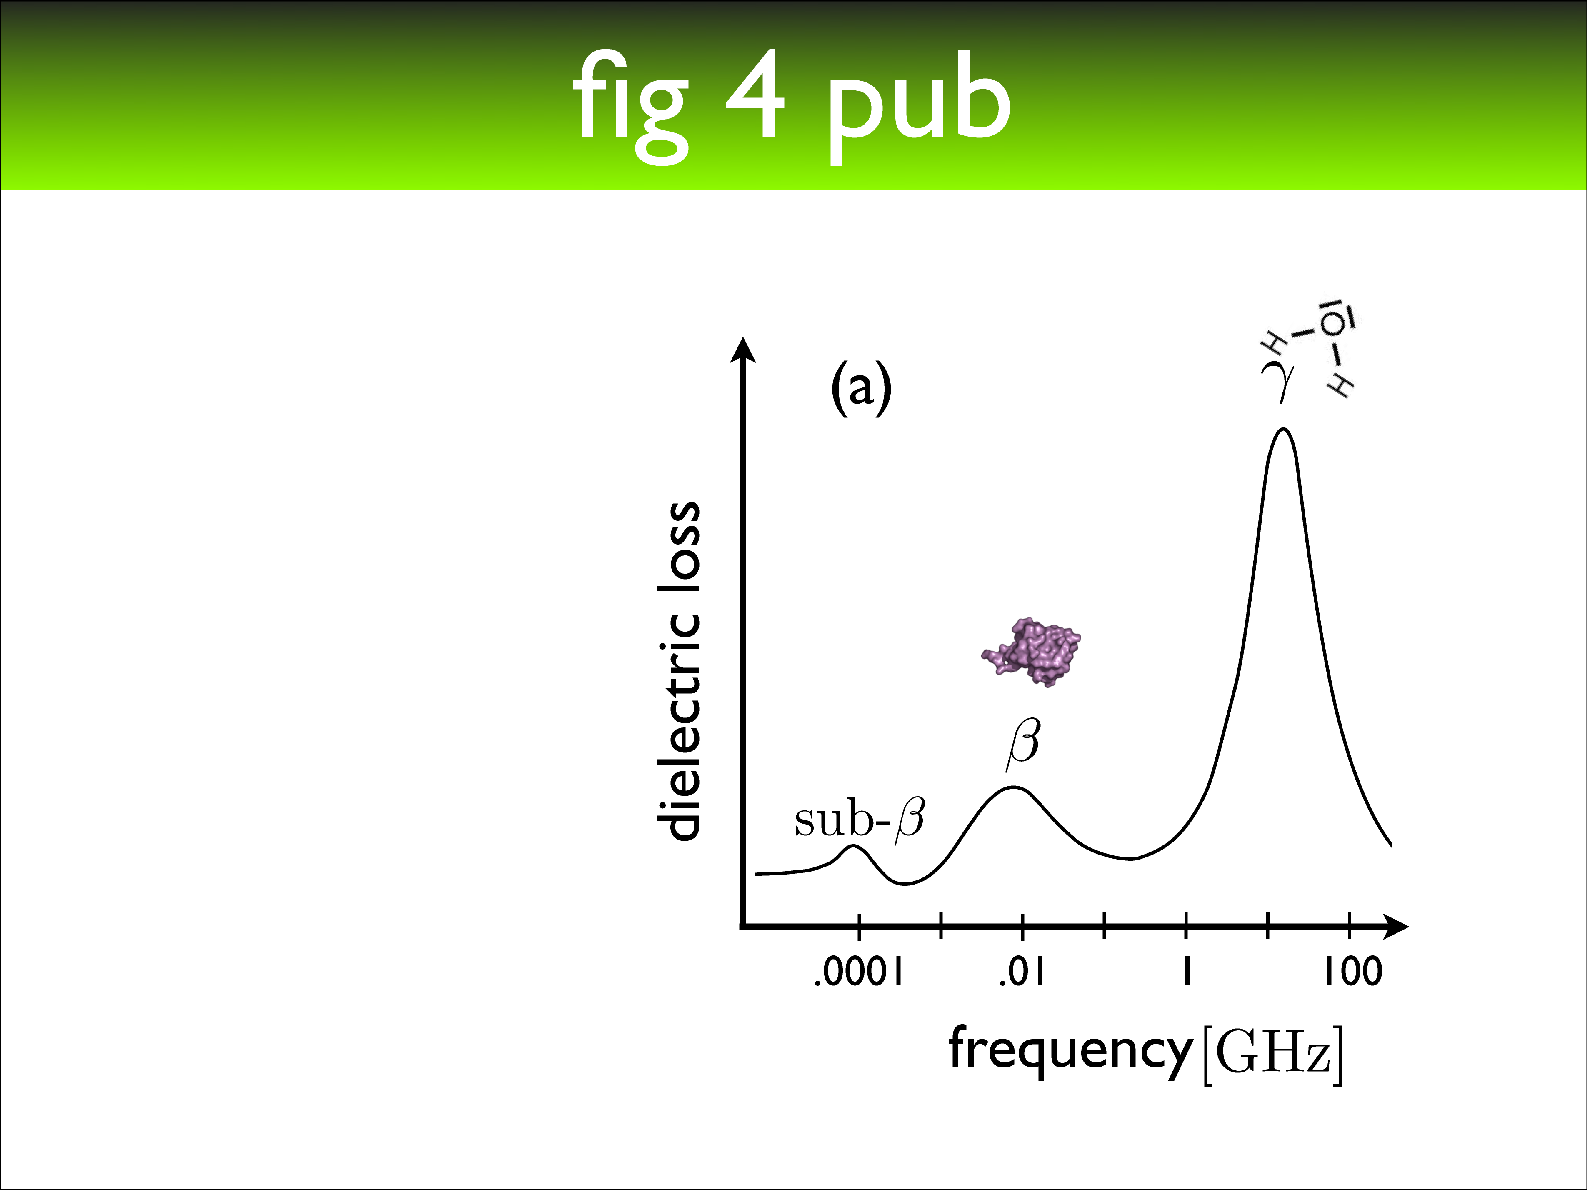
\includegraphics[clip=true,
 % % %   pdf  % % % trim= 12.5cm 2.1cm 4.4cm 5.5cm,
 trim = 11cm 1.7cm 3cm 5cm,
 width=3.45cm]
 {figuresPRL/DRS_FEM_BEM_wSciPAL_fig1a_simple-DRS-loss-spectrum-eps-converted-to.pdf}
% DRS_FEM_BEM_wSciPAL_fig1a_simple-DRS-loss-spectrum-eps-converted-to.pdf}
 \label{DRS_FEM_BEM_wSciPAL-fig:diel-loss-spec}
 }
 %
 \subfloat
 {
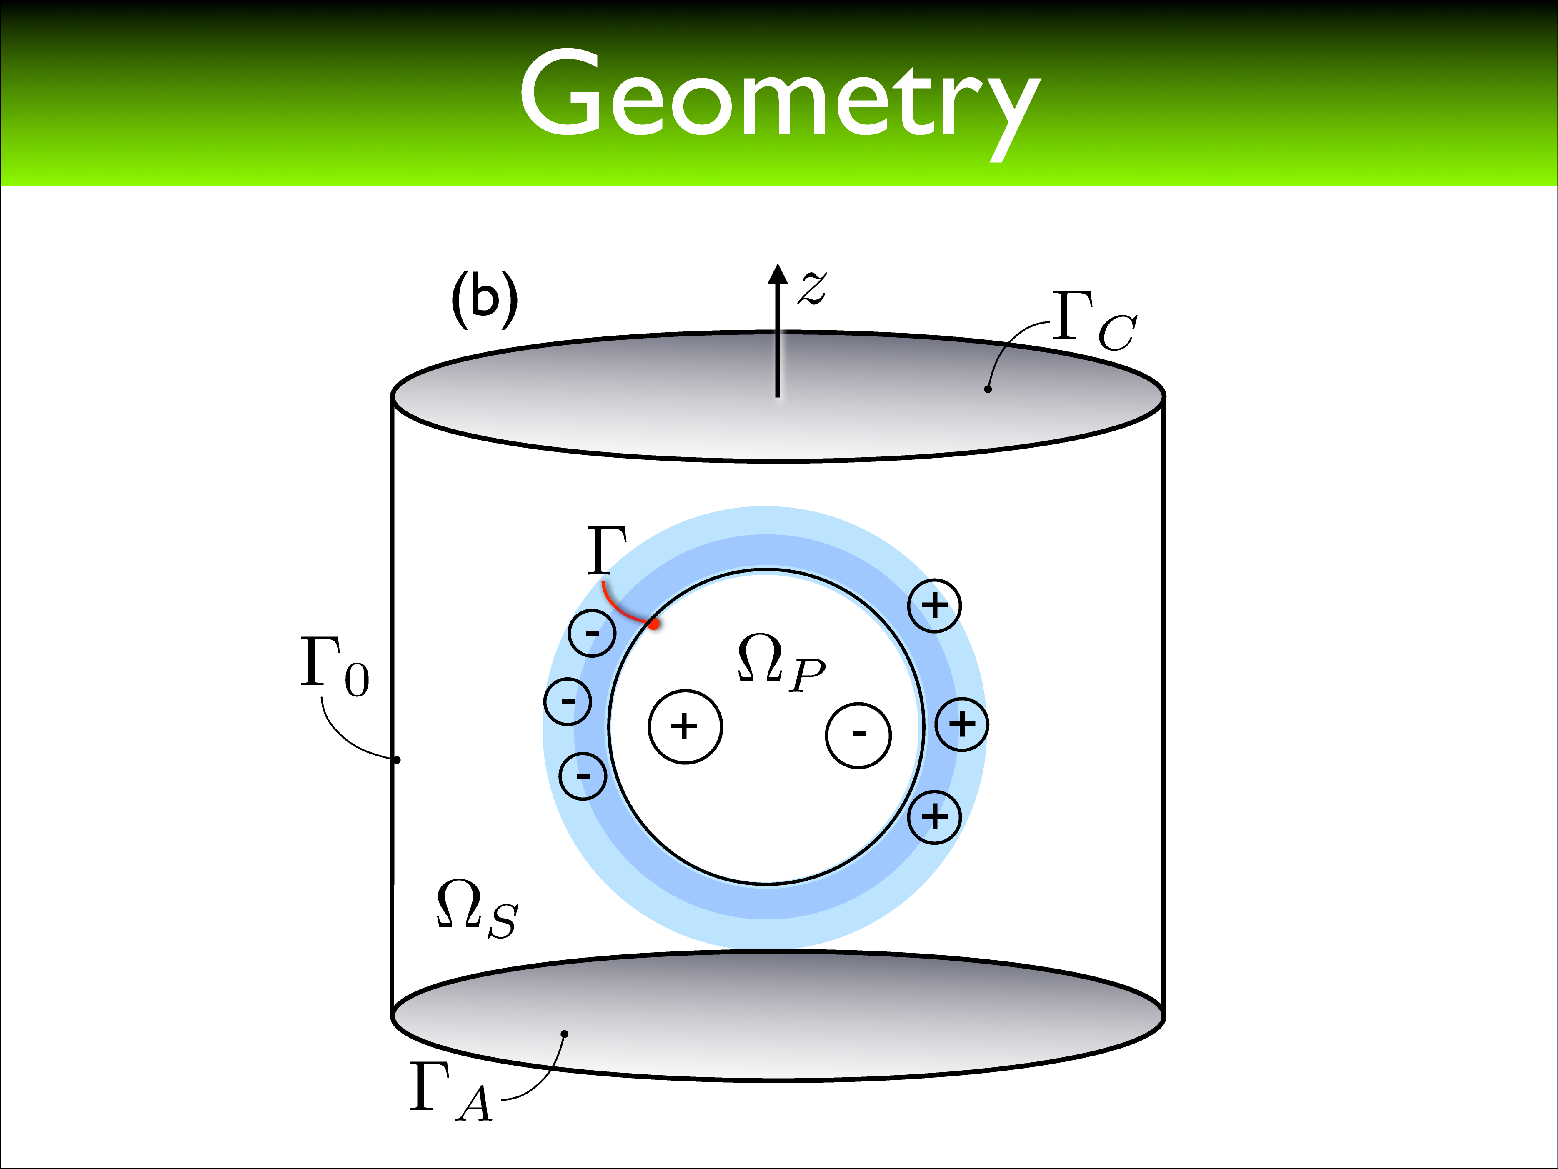
\includegraphics[clip=true,
 % % %   pdf  % % % trim=6.7cm 1.25cm 8.25cm 5cm,
 trim = 5.1cm 0.75cm 6.5cm 4.5cm,
 width=3.7cm]
 {figures-PRL/DRS_FEM_BEM_wSciPAL_fig1b_drs-setup-and-effect-eps-converted-to.pdf}
\label{DRS_FEM_BEM_wSciPAL-fig:protein-state-a}
}
 %
 \subfloat
 {
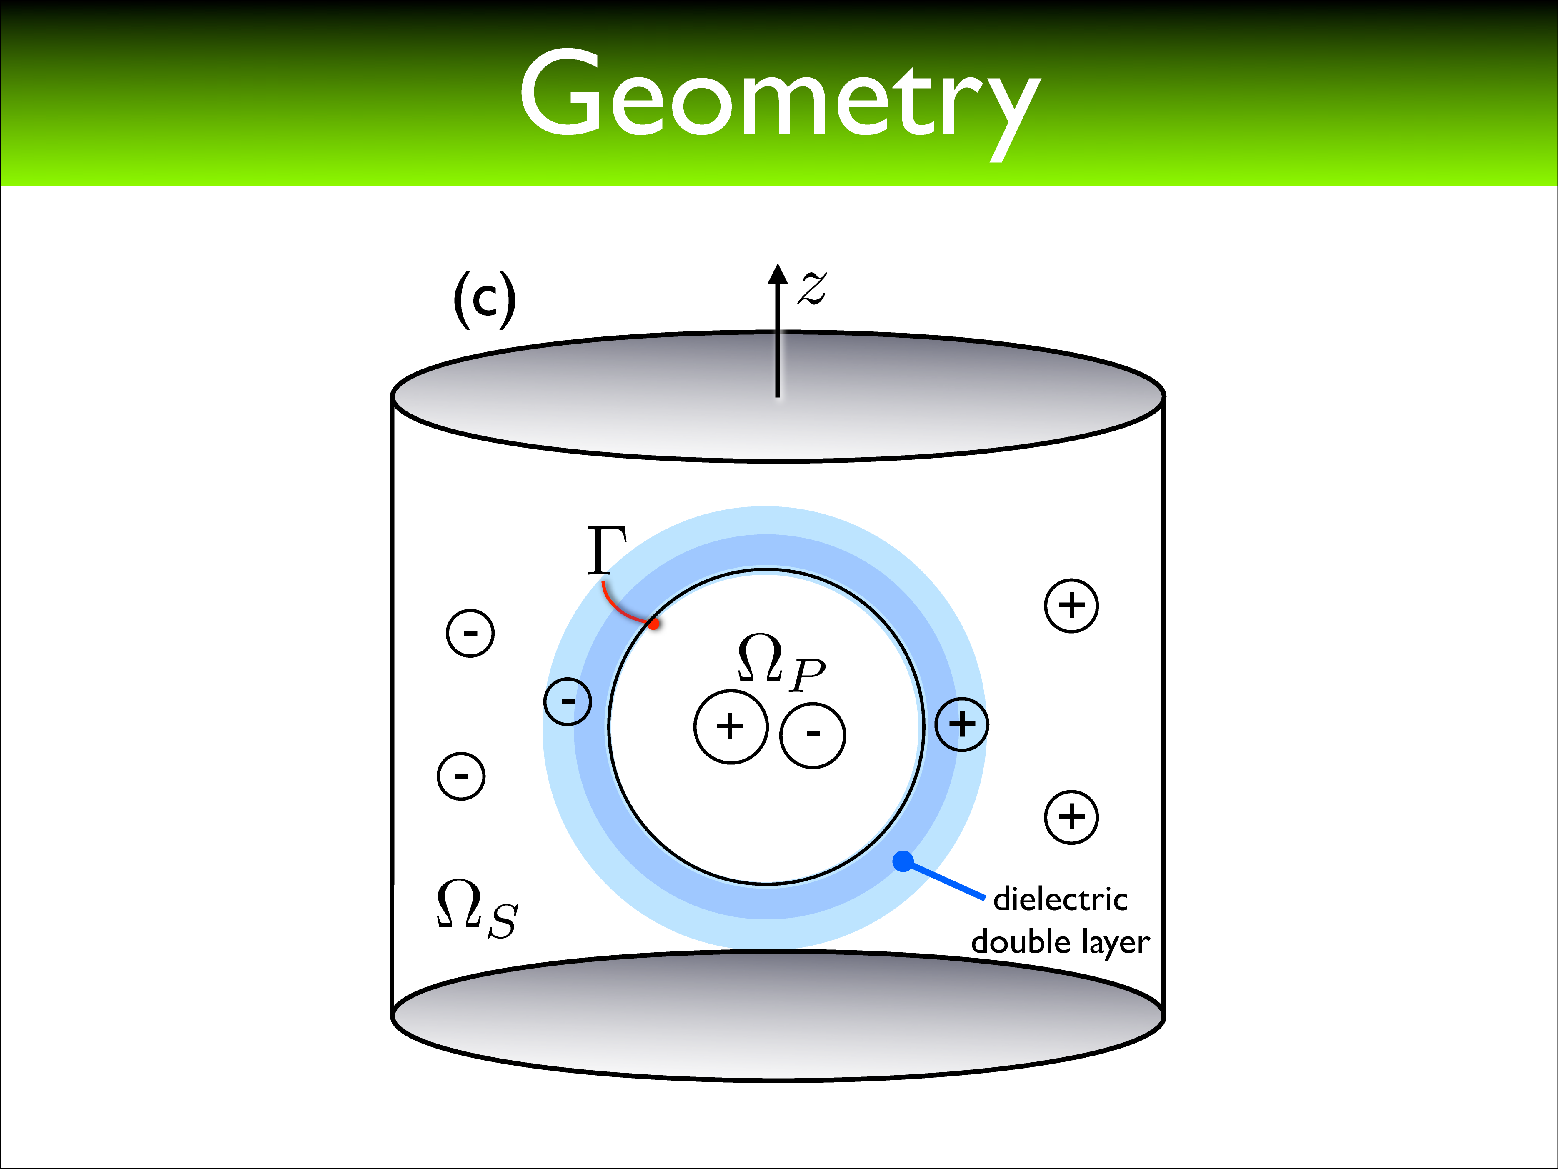
\includegraphics[clip=true,
% % %   pdf  % % %  trim=6.7cm 1.25cm 8.25cm 5cm,
 trim = 5.1cm 0.75cm 6.5cm 4.5cm,
 width=3.7cm]
 {figures-PRL/DRS_FEM_BEM_wSciPAL_fig1c_drs-setup-and-effect-eps-converted-to.pdf}
 \label{DRS_FEM_BEM_wSciPAL-fig:protein-state-b}
 }
%
%If the width of the figure is less than 7.8 cm use the \texttt{sidecaption} command to flush the caption on
\caption{
\mydiff{
DRS cell with subdomains $\Omega_P$ (protein interior) and $\Omega_S$ (solvent). 
%
The boundaries are $\Gamma$ (protein-solvent interface),  $\Gamma_A$ (anode), $\Gamma_C$ (cathode) and $\Gamma_0$ (impermeable hull of the DRS cell). 
%
The protein is modeled as a dipole consisting of two point charges immersed in a spherical, dielectric domain of relative permittivity $\varepsilon_P \approx 2$ while the aqueous surrounding has $\varepsilon_S \approx 80$. 
%
Depending on the intramolecular charge distribution, i.e.  conformation, of the protein a different number of ions is bound in the dielectric double layer at $\Gamma$. 
}
% % % % % % % % % % % NEW CAPTION % % % % % % %
{(a) Dielectric loss spectrum of ubiquitin.
(b,c) Charge configurations in protein (domain $\Omega_P$) in the DRS cell $\Omega = \Omega_S \cup \Omega_P$.
%, formed by the protein interior $\Omega_P$ and the solvent domain $\Omega_S$. 
%
%The protein-solvent interface is $\Gamma = \overline{\Omega_S} \cap \overline{\Omega_P}$.
%
Details see text.
}
}
\label{DRS_FEM_BEM_wSciPAL-fig:drs-setup-and-effect}    
\end{figure}


A realistic description of 
% % % post review change 
% the DRS experiment 
DRS
requires BCs for the ${\bf j}_a$  and $\Phi$ capable of modeling an applied current. 
%
Usually, the redox reaction rates $K_R$ and $K_O$ are described by
Butler-Volmer kinetics, %~\cite{X}, 
including the Frumkin correction
%~\cite{X}
 due to the Stern layer~\cite{schmickler2010interfacial}.
% 
%As already pointed out in~\cite{BazantPhysRevE.70.021506} the BCs for "ideally polarizable" or "completely blocking" electrodes can be simplified to a Robin-type condition.
%%
%Furthermore, we adopt the simplified Tafel kinetics~\cite{schmickler2010interfacial}, which
%neglects oxidation (reduction) processes at the cathode (anode)
%completely. Since we are not interested in diffuse-charge effects at the electrodes we can use the limit of a vanishing thickness of the Stern layer.
%
% With these simplifications
As discussed \mydiff{elsewhere}{in}~\cite{kramer2012cuda}, for $\Phi$ \mydiff{simple Dirichlet}{Dirichlet} BCs,
%
%\begin{equation}
$\Phi\big|_{\Gamma_C} = \Phi_C$, % \quad
$ \Phi\big|_{\Gamma_A}=\Phi_A $, suffice. % \,.
%\end{equation}    
%
The redox reaction implies a balance of \mydiff{inward}{in-} and outward fluxes
% % % post review change
%of the current transferring species 
at the electrodes
%
\begin{eqnarray}
\label{DRS_FEM_BEM_wSciPAL-eq:currentcathodebc}
{\bf n} \cdot {\bf j}_+\big|_{\Gamma_C} & = &  K_R~c_+\big|_{\Gamma_C}   =~ -{\bf n}  \cdot {\bf j}_0\big|_{\Gamma_C} \,, \\
%
\label{DRS_FEM_BEM_wSciPAL-eq:currentanodebc}
 -  {\bf n} \cdot {\bf j}_+\big|_{\Gamma_A}
  & = & K_O ~ c_0\big|_{\Gamma_A} ~= ~{\bf n} \cdot {\bf j}_0\big|_{\Gamma_A} \,,
\end{eqnarray}
%
where ${\bf n}$ is the outer normal of the surface $\partial\Omega_S$
 and $\cdot |_{B}$ is the trace on some part $B\subset \partial \Omega_S = \Gamma_C \cup \Gamma_0 \cup \Gamma_A \cup \Gamma$.
%
The rates are treated as constants, especially \mydiff{the}{their} dependence on~$\Phi$ is neglected.
%
The anions do not contribute to the current transport and fulfill
%
% \begin{equation}
$ {\bf n} \cdot{\bf j}_-|_{\Gamma_A} 
=
 {\bf n} \cdot{\bf j}_-|_{\Gamma_C} 
   =0 % \,.
%\end{equation} 
$.
%
The hull $\Gamma_0$ of the cell and the protein surface $\Gamma$ are impermeable for all ions,
%
%\begin{equation}
 $ {\bf n} \cdot{\bf j}_a|_{\Gamma_0} 
 =
 {\bf n} \cdot{\bf j}_a|_{\Gamma} 
   =0$, 
   %    \quad 
   $  a \in \{+,0,-\} %\,.
$.
%\end{equation} 
%
For $\Phi$ we have ${\bf n} \cdot \nabla \Phi|_{\Gamma_0} = 0$ and~$\Gamma$ is 
% % % post review change
% not a boundary, but 
a dielectric interface with 
% % % post review change
% the
continuity and the jump relations
% 
\begin{eqnarray}
\label{DRS_FEM_BEM_wSciPAL-eq:dPhi-jump}
\lim_{\delta \to 0} \Phi ( {\bf x} - \delta {\bf n} )  =  \lim_{\delta\to 0} \Phi ( {\bf x} + \delta {\bf n})  \,, 
&~~~&
%\mydiff{\lbrack \varepsilon( {\bf x}) {\bf n}\cdot\nabla\Phi \rbrack  =  0. }{
 \varepsilon_P( {\bf x}) {\bf n}\cdot\nabla\Phi ~=~ \varepsilon_S( {\bf x}) {\bf n}\cdot\nabla\Phi
 \quad \forall {\bf x} \in \Gamma\,.
% }
\end{eqnarray}
%
% \mydiff{An immediate consequence of these is that ions and the potential have different computational domains.} {}
%
% % % post review change
%There are quite some efforts in 
One goal in computational biochemistry is to \mydiff{accurately}{} model molecular surfaces of proteins in a smooth manner~\cite{Bajaj20091684}.
%
% % % post review change
% Hence, instead of striving for
Instead of an accurate sub-cell resolution of the dielectric interface~$\Gamma$
we 
% % % post review change
% rather 
\mydiff{opt for converting}{convert} the interior constant-coefficient-Poisson equation into a
boundary integral equation (BIE) on $\Gamma$.
%
\mydiff{Thus, the}{The} protein becomes an excluded volume $\Omega_P$ of constant dielectric permittivity $\varepsilon_r = \varepsilon_P$ containing point charges~$\{q_k\}$ at fixed positions~$ \{ {\bf x}_k \}$.
%
To do this, we apply the discussion of the BIE formulation for linear interior Neumann boundary value and interface problems in~\cite{Rjasanow2007book}.
%
\mydiff{To use the}{The} Johnson-N\'ed\'elec 
coupling~\cite{johnson1980coupling} \mydiff{we introduce}{needs} the normal component of the electric field w.r.t. to the outer normal ${\bf n}_P$ (${\bf n}_P = -{\bf n}$ on $\Gamma$) of $\Omega_P$ as independent variable
%
%\begin{equation}
$ t^P   :=  -\partial_{{\bf n}}\Phi $.  %\,.
%\end{equation}
%
\mydiff{new paragraph}{
% % % post review change
%From potential theory follows that for
Potential theory shows that on $C^1$-smooth, closed surfaces~$\Gamma$ the intramolecular 
% % % post review change
% contribution $\Phi_P$ to
part $\Phi_P$ of the potential at ${\bf x} \in \Gamma$ fulfills
% 
\begin{eqnarray*}
\label{DRS_FEM_BEM_wSciPAL-eq:phi-at-gamma-ps}
\frac 1 2 \Phi ({\bf x})  & + &
\oint_{\Gamma}
\left[
\Phi ({\bf x}' ) \frac{\partial G_{\bf x} }{\partial{\bf n}'_P}({\bf x}') 
 - 
 G_{\bf x}({\bf x}')  % \frac{\varepsilon_S}{\varepsilon_P} 
    \frac{\partial \Phi}{\partial{\bf n}'_P} ({\bf x}')   \right] 
 d\Gamma ({\bf x}')  
% \nonumber \\
 %& = &
  =  \frac{1}{\varepsilon_P}  \int_{\Omega_P}  G_{\bf x}({\bf x}')  \rho_f({\bf x}')  \,.
  \quad 
\end{eqnarray*}
% 
Here, $G_{\bf x}({\bf y}) := 1 / (4 \pi |  {\bf x} - {\bf y} | )  $
%
is the Green's function of the Laplace equation. % in three dimensions. 
The right-hand side defines the Newton potential $\phi^C$. % ( {\bf x})$.
%
% \begin{equation}
%$
%\phi^C ( {\bf x}) =   % \frac{1}{
%(4 \pi \varepsilon_P)^{-1}
%%} 
%\sum_k    q_k / |  {\bf x} - {\bf x}_k |   % \frac{q_k}{|  {\bf x} - {\bf x}_k | } % \,. 
%$  due to the \mydiff{intramolecular charges}{}~$\{q_k\}$.
%
We define the single layer boundary integral operator (BIO) $V : H^{-1/2}(\Gamma) \to H^{1/2}(\Gamma) $ and the double layer BIO $K : H^{1/2}(\Gamma) \to H^{1/2}(\Gamma) $ as
 % % % post review change
%usual 
in \cite[Secs. 6.2 and 6.4]{steinbach2007numerical}.
% % % post review change
%but 
Instead of ${\bf n}_P$ we use the outward normal ${\bf n} = -{\bf n}_P$ relative to $\Omega_S$
% 
\begin{eqnarray*}
(V t^P)({\bf x})  :=  \oint_{\Gamma}
%\left[
 G_{\bf x}({\bf x}')  % \frac{\varepsilon_S}{\varepsilon_P}  
   %\frac{\partial \Phi}{\partial{\bf n}'}
     t^P({\bf x}')
 %    \right] 
 d\Gamma ({\bf x}')  \,,& ~~~~~~& 
%
(K \Phi_P)({\bf x})  :=  % -
\oint_{\Gamma}
%\left[
\frac{\partial G_{\bf x} }{\partial{\bf n}({\bf x}') }({\bf x}') 
 % \frac{\varepsilon_S}{\varepsilon_P}  
     \Phi({\bf x}')
  %   \right] 
 d\Gamma ({\bf x}')  \,.
\end{eqnarray*}
%
}
From Eq.(\ref{DRS_FEM_BEM_wSciPAL-eq:dPhi-jump}) follows
%
% 
%\begin{eqnarray}
$
\varepsilon_S  \partial_{\bf n} \Phi \big|_{\Gamma} = -\varepsilon_P  t^P $ and we get
%\end{eqnarray}
%
%Then, at a point ${\bf x}$ on a sufficiently smooth surface~$\Gamma$ the potential $\Phi$ fulfills
%
%\begin{eqnarray}
%\label{DRS_FEM_BEM_wSciPAL-eq:phi-at-gamma-ps}
%\frac 1 2 \Phi ({\bf x})  & + &
%\oint\limits_{\Gamma}
%\left[
%\Phi ({\bf x}' ) \frac{\partial G_{\bf x} }{\partial{\bf n}'_P}({\bf x}') 
% - 
% G_{\bf x}({\bf x}')  % \frac{\varepsilon_S}{\varepsilon_P} 
%    \frac{\partial \Phi}{\partial{\bf n}'_P}  \right] 
% d\Gamma ({\bf x}')  
%% \nonumber \\
% %& = &
%  =  \frac{1}{\varepsilon_P}  \int_{\Omega_P}  G_{\bf x}({\bf x}')  \rho_P({\bf x}')  %  d^3x'
%  \quad 
%\end{eqnarray}
%
\begin{eqnarray}
\label{DRS_FEM_BEM_wSciPAL-eq:JN-strong}
   \left( \frac 1 2 I  -
    K  \right)\Phi %\big|_{\Gamma}
    + % "+" is for the formulation w d_n Phi
 \frac{\varepsilon_S}{\varepsilon_P} 
 %(\varepsilon_S /\varepsilon_P )
  V % \partial_{\bf n} \Phi  \big|_{\Gamma} 
  t^P
  & = &  \phi^C \,.
\end{eqnarray}
% 
\mydiff{where we define
%
$G_{\bf x}({\bf y}) := 1 / (4 \pi |  {\bf x} - {\bf y} | )  $
%
as Green's function. % for the Laplace equation in three dimensions.
%
The Newton potential due to the~$\{q_k\}$ is
%
% \begin{equation}
$
\phi^C ( {\bf x}) =   % \frac{1}{
(4 \pi \varepsilon_P)^{-1}
%} 
\sum_k    q_k / |  {\bf x} - {\bf x}_k |   % \frac{q_k}{|  {\bf x} - {\bf x}_k | } % \,. 
$. 
% \end{equation}
%
%
The single layer boundary integral operator (BIO) $V : H^{-1/2}(\Gamma) \to H^{1/2}(\Gamma) $ and double layer BIO $K : H^{1/2}(\Gamma) \to H^{1/2}(\Gamma) $ are defined as usual \cite[Secs. 6.2 and 6.4]{steinbach2007numerical}.
% 
%\begin{eqnarray}
%(V t^P)({\bf x}) & = & \oint\limits_{\Gamma}
%%\left[
% G_{\bf x}({\bf x}')  % \frac{\varepsilon_S}{\varepsilon_P}  
%   %\frac{\partial \Phi}{\partial{\bf n}'}
%     t^P({\bf x}')
% %    \right] 
% d\Gamma ({\bf x}')  \,, \\
%%
%(K \Phi_P)({\bf x}) & = & % -
%\oint\limits_{\Gamma}
%%\left[
%\frac{\partial G_{\bf x} }{\partial{\bf n}({\bf x}') }({\bf x}') 
% % \frac{\varepsilon_S}{\varepsilon_P}  
%     \Phi({\bf x}')
%  %   \right] 
% d\Gamma ({\bf x}')  \,.
%\end{eqnarray}
%
%The operator $V : H^{-1/2}(\Gamma) \to H^{1/2}(\Gamma) $ is bounded and $H^{-1/2}(\Gamma)$-elliptic and thus invertible.
%
%
This introduces a FEM-BEM method for the potential.
}{This is the basis for the FEM-BEM method for the potential, 
% % % post review change
% such that the
reducing its
computational domain
% % % post review change
% for the potential $\Phi$ is reduced 
to $\Omega_S = \Omega \backslash \Omega_P$.}
%
The distribution of the 
% % % post review change
% other species
ions 
is governed by convection-diffusion equations with either Neumann or Robin but no Dirichlet BCs.
%
The link to experiments is 
% % % post review change
%given by 
the direct current $I_{dc}$ created by a potential difference $\eta := \Phi_C - \Phi_A$.
%
Due to the redox reaction at the electrodes
% % % post review change
% the current is
% 
%\begin{equation}
$
I_{dc} 
=
 \int_{\Gamma_C}  {\bf n} \cdot{\bf j}_+ d\Gamma_C
  =
   K_R \int_{\Gamma_C}  c_+ d\Gamma_C$. % \,.
%\end{equation}
%
The conformational sampling introduces a time-dependence on $I_{dc}$. 
%
This is modeled by a two-state telegraph process,
%
\mydiff{}{ %
% % % post review change
% This simplifies the time dependence to 
i.e. a random
switching between two stationary states.
% % % post review change
% and 
This makes Eq.(\ref{DRS_FEM_BEM_wSciPAL-eq:model_a}) formally time independent. For details cf. \cite{kramer2012cuda}.}
%
% % % post review change
%Hence, t
To validate the hypothesis about the origin of the ``sub-$\beta$'' peak we 
% % % post review change
%merely 
have to compute two different values for $I_{dc}$ from the time independent version of Eq.(\ref{DRS_FEM_BEM_wSciPAL-eq:PDE-model}).


\section{Weak Formulation and Discretization}
\label{DRS_FEM_BEM_wSciPAL-sec:drs-fem-bem-weak-form}

\mydiff{}{
We do not solve Eq.(\ref{DRS_FEM_BEM_wSciPAL-eq:PDE-model}) in its mixed form, but reduce it to a set of convection-diffusion equations by inserting Eq.(\ref{DRS_FEM_BEM_wSciPAL-eq:currents}) into Eq.(\ref{DRS_FEM_BEM_wSciPAL-eq:model_a}), eliminating the currents.
% % % post review change
% as independent unknowns.
}

Let $(\cdot, \cdot)_D$ be the $L^2$ inner product on a domain $D$ and $\| \cdot \|_X$ the norm of a function space $X$.
%
For $D \equiv \Omega_S$ we drop the index.
%
The weak 
% % % post review change
% formulation 
form of Eq.(\ref{DRS_FEM_BEM_wSciPAL-eq:PDE-model}) is derived 
% % % post review change
%as usual 
by multiplying with test functions, integrating by parts and inserting all flux BCs.
%
%we first have to specify the function spaces in which we search for the solution.
%Inserting the BCs for the fluxes we get 
%
%\begin{subequations}
%\begin{eqnarray}
%\label{DRS_FEM_BEM_wSciPAL-eq:generic-adr-fem-c+}
%(\nabla s, \nabla c_+) + (\nabla s, c_+ \nabla \Phi)  % && \nonumber \\
%  +  k_R( s,  c_+ )_{\Gamma_C} 
% - k_O ( s, c_0 )_{\Gamma_A} 
%%
% & = & 0 \quad \\
%% \nonumber \\
% \label{DRS_FEM_BEM_wSciPAL-eq:generic-adr-fem-c0}
% - k_R ( u, c_+ )_{\Gamma_C} +
%(\nabla u, \nabla c_0)  % && \nonumber \\
% + k_O ( u,   c_0 )_{\Gamma_A}  
%%
% & = & 0 \quad \\
%% \nonumber \\
% \label{DRS_FEM_BEM_wSciPAL-eq:generic-adr-fem-c-}
%(\nabla v, \nabla c_-) - (\nabla v, c_- \nabla \Phi)  
%% - ( v,  \partial_{{\bf n}}  c_- - c_- \partial_{{\bf n}} \Phi )_{\Gamma_S} 
%%
% & = & 0 \quad \\
%  %\nonumber \\
% \label{DRS_FEM_BEM_wSciPAL-eq:generic-adr-fem-phi}
%  - ( w, c_+ - c_- ) +
% \varepsilon_S (\nabla w, \nabla \Phi)%   && \nonumber \\
%+
%  \varepsilon_P ( w,  t^P )_{\Gamma} 
%% - ( w,   \partial_{{\bf n}} \Phi )_{\Gamma_S} 
%%
% & = & 0  %(w,\varrho_P)_{ \Omega_P} 
%  \quad \quad \\
%%    \nonumber \\
%    \label{DRS_FEM_BEM_wSciPAL-eq:generic-adr-fem-tp}
%    \left(\psi, \left(\frac 1 2  I  - K \right) \Phi \right)_{\Gamma} % && \nonumber \\
%    + 
%      \frac{\varepsilon_S}{\varepsilon_P}  \left(\psi,   V t^P \right)_{\Gamma}  
%    & = & 
%% \frac{1}{\varepsilon_P}  
%\left(\psi, \phi^C \right)_{\Gamma} \,. \quad  \quad 
%\end{eqnarray}
%\end{subequations}
%
% A suitable function space for the solution is composed as follows.
%
The Dirichlet BCs for the potential $\Phi$ 
% % % post review change
%on the electrodes 
are built into the solution space $X$
for the FEM part.
%
We define~$X$ as a direct product of a space~$X^c := [H^1(\Omega_S)]^3  $ for the densities and 
% % % post review change
%a separate~
$X^{\Phi} :=  \{   \Phi \in H^1(\Omega_S) : ~ \Phi|_{\Gamma_A} = 0, ~\Phi|_{\Gamma_C} = \eta   \} $ for $\Phi$.
% 
For the BCs for $\Phi$ on $\Gamma$ we need
% % % post review change
%a separate 
the space $Y := H^{-1/2}(\Gamma)$.
% % % post review change
% so that t
The final solution space is $V := X \times Y$.
%
%\begin{eqnarray*}
%X^c & := & [H^1(\Omega_S)]^3   \,, \\
% X^{\Phi}  & := & \{   \Phi \in H^1(\Omega_S) : ~ \Phi|_{\Gamma_A} = 0, ~\Phi|_{\Gamma_C} = \eta   \} \,, \\
% X & = & X^c \times X^{\Phi} 
% \,, \\
%\label{DRS_FEM_BEM_wSciPAL-eq:full-space}
%V & := & X \times Y\,.
%\end{eqnarray*}
%
The FEM part of the solution is
${\bf u} :=  (c_{+}, c_{0}, c_{-}, \Phi)
$
and the test function is~${\bf v} := (s,u,v,w)$. 
%
 \ifthenelse {\boolean{IsRelease}}{\subsubsection*{structure of the algebraic system}}{}
%
Except for the interface term for $\Phi$ on $\Gamma$ the weak form 
% % % post review change
%can be recast into 
is
a semilinear form 
$
a(\cdot; \cdot) : X \times X \to \mathbb{R}
$
 which is nonlinear in its first argument.
%
The terms in $a(\cdot; \cdot) $ can be grouped to reflect, after linearizing, the block structure of the matrix 
% % % post review change
% by interpreting the 
using 
scalar test functions as block row and 
% % % post review change
%the 
trial functions as block column indexes.
%
Diagonal terms are 
% % % post review change
% contained 
in $a_D(\cdot; \cdot) $, linear upper off-diagonal terms in $a^{l}_U(\cdot; \cdot) $, nonlinear drift terms in $a^{d}_U(\cdot; \cdot) $ and lower off-diagonal terms in $a_L(\cdot; \cdot) $, i.e.
\begin{eqnarray*}
a_D({\bf u}; {\bf v}) & := & (\nabla s, \nabla c_+)  + 
(\nabla u, \nabla c_0)  % && \nonumber \\
 + k_O ( u,   c_0 )_{\Gamma_A} 
 +
 (\nabla v, \nabla c_-) 
 +
  \varepsilon_S (\nabla w, \nabla \Phi), \\
  %
a^{l}_U({\bf u}; {\bf v}) & := & - k_O ( s, c_0 )_{\Gamma_A}  \,, \quad
% \\
  %
a^{d}_U({\bf u}; {\bf v}) ~ := ~  (\nabla s, c_+ \nabla \Phi) - (\nabla v, c_- \nabla \Phi)  \,,
\\
a_L({\bf u}, {\bf v}) & := &  - k_R  ( u, c_+ )_{\Gamma_C}   - ( w, c_+ - c_- ) \,.
\end{eqnarray*}
%
After linearizing $a^{d}_U( \cdot; \cdot ) $ w.r.t. $c_+$ and $c_-$, the associated matrices are $A_D$, $A_U$ and $A_L$, respectively. %, and we define $A := A_L + A_D + A_U $.
%
The left-hand side of the weak form of Eq.(\ref{DRS_FEM_BEM_wSciPAL-eq:JN-strong}), with associated matrices $B_K$ and $B_V$,  is a sum of the two bilinear forms
\begin{eqnarray*}
b_K(\psi, \Phi)
 ~ := ~& 
     \left(\psi, \left(\frac 1 2  I  - K \right) \Phi \right)_{\Gamma}  & ~ :  ~H^{1/2}(\Gamma)  \times H^{1/2}(\Gamma) \to \mathbb{R} \,, \\
    %
b_V(\psi, t^P)
  ~:= ~& \frac{\varepsilon_S}{\varepsilon_P}  \left(\psi,   V t^P \right)_{\Gamma} & ~: ~ H^{-1/2}(\Gamma) \times H^{1/2}(\Gamma) \to \mathbb{R} \,.
\end{eqnarray*}
%
%
We use conformal discretizations $ X_h \subset X$ and $ Y_h \subset Y$ by globally continuous Lagrange elements for which we use  deal.II's \verb|FE_Q<dim>| class.
%
In practice, the trial functions in $Y_h$ are given by the traces of those in $X_h$ because we treat the normal derivative as independent variable. 
%
This is due to the way finite elements are implemented in deal.II. 
%
The same holds for the test functions $\psi$ in the dual space $Y'_h \subset H^{1/2}(\Gamma)$.
Then, the discretized variational problem is: 
$Find ~({\bf u}_h, t^P_h) \in X_h \times Y_h ~s.~t.$
% 
\begin{subequations}
\label{DRS_FEM_BEM_wSciPAL-eq:discrete-nl-var-form}
\begin{eqnarray}
 %&
 \forall {\bf v}_h \in X_h~: ~% \hspace{3.2cm} &  \\
& a ({\bf u}_h; {\bf v}_h) +
 ( w,  \varepsilon_P t^P )_{\Gamma} & = ~ 0 \,,  \\
 %\nonumber \\
 %&
  \forall \psi_h \in Y'_h ~: ~ % \hspace{3.2cm} &  \\
  & b_K(\psi_h, \Phi_h) % \left(\psi, \left(\frac 1 2  I  - K \right) \Phi \right)_{\Gamma}
    + 
     b_V(\psi_h,  t^P_h) % \left(\psi,  \frac{\varepsilon_S}{\varepsilon_P}   V t^P \right)_{\Gamma}  
    & = ~
% \frac{1}{\varepsilon_P}  
\left(\psi_h, \phi^C \right)_{\Gamma}  \,.  
\end{eqnarray}
\end{subequations}
%
\ifthenelse {\boolean{IsRelease}}{\subsubsection*{Discretization}}{}
%
% % % post review change
% When solving the discretized problem we encounter several numerical problems.
Several numerical problems arise in solving the discretized problem.
%
Only the potential $\Phi$ is unambiguous since it is subject to Dirichlet BCs 
% % % post review change
% on some part of the boundary 
at the electrodes $\Gamma_A$ and $\Gamma_C$.
%
The equation for the density of the neutral particles $c_0$ effectively is a pure Neumann Laplace problem. 
%
Its average merely enters via the boundary terms in Eq.(\ref{DRS_FEM_BEM_wSciPAL-eq:currentanodebc}) for the cations $c_+$.
%
% % % post review change
% Due to the stationary state the p
Particle numbers,
% % % post review change
and thus average densities,
%
are conserved
$\int_{\Omega_S} c_a ~d \Omega_S  = const$, $a \in \{+,0,-\}$
%
in the stationary state.  % % % order changed post review
%
% % %  post review change
% The conservation of the average densities is enforced by introducing
This
is enforced by adding a pseudo-time dependence, i.e.
% % % post review change
% , i.e. adding a scaled identity to the Laplace operator. 
%
% % % post review change
% Since we are looking for stationary states this corresponds to ``adding a 0", i.e.
% % % post review change
% after time discretization
%
$ -\nabla^2u = f  $ becomes $[\delta I -\nabla^2] u^{n+1} = f + \delta u^n$,
% % % post review change
%  after time discretization.
%
where
% % % post review change
% The small parameter 
$\delta$ 
% % % post review change 
% plays the role of 
is
an inverse time step and $I$ is the identity operator.

We solve by interleaving successive mesh refinement, pseudo-time stepping and reassembly of the nonlinear terms. 
%
This introduces a sequence of finite-dimensional subspaces ${X_h} \subset X$, parametrized by the cell diameter $h$.
%
% % % post review change
% % Then, o
On a given mesh, i.e. in FE space $V^{\ell}_h \subset V$,  $V^{\ell}_h \subset V^{\ell+1}_h $ we run a few steps in pseudo-time (while $\|u^{n+1} - u^{n} \|_{\ell_2} \ge Tol$).
%
In each time step we reassemble the drift terms in $A_U$ after solving the linear algebraic problem by deal.II's GMRES solver with left-preconditioning.
%
 \ifthenelse {\boolean{IsRelease}}{\subsubsection*{numerical solution}}{}

For the numerical solution of Eq.(\ref{DRS_FEM_BEM_wSciPAL-eq:discrete-nl-var-form}) we have considerably extended the GMG example {\sf step-16} of deal.II, v7.2.0. 
%
%
When computing the matrices $B_K$, $B_V$ from the bilinear forms $b_K(.,.)$ and $b_V(.,.)$ the double integration is avoided by using the support points of the test functions for collocation.
%
With $t^P_h = \sum_i t^P_i \phi_i\in Y_h$, e.g. the entries of the matrix representing the single layer BIO are formally given by
$
B_{V,ij} = (\psi_i , V \phi_j ).
$ 
Let ${\bf x}_i$ be the support point of DoF~$i$, then collocation at ${\bf x}_i$ can be interpreted as 
$
B_{V,ij} = (\delta ({\bf x} - {\bf x}_i) , V \phi_j )
$,
i.e. $B_{V,ij}$ is % and $K_{ij}$ are
 computed as 
\begin{eqnarray}
B_{V,ij} & = & \oint_{\partial \Omega_S}
%\left[
 G_{{\bf x}_i}({\bf x}') 
     \phi_j({\bf x}')
 %    \right] 
 d\Gamma ({\bf x}')  % \,, \\
%
%K_{ij} & = & % -
%\oint\limits_{\partial \Omega_S}
%\frac{\partial G_{{\bf x}_i} }{\partial{\bf n}({\bf x}') }({\bf x}') 
%     \phi_j({\bf x}')
% d\Gamma ({\bf x}')  
\,.
\end{eqnarray}
%
\section{Assembly and Preconditioning}
%

\begin{itemize}
\item the class \lstinline|FemBemProblem| drives the memory management, matrix assembly, setup of preconditioners, solving the linear algebraic system, data output including postprocessing for computing physical observables and mesh refinement.
%
To facilitate the quick implementation of different variations of the PNP equations it provides internal classes \lstinline|SparsityPatternSet| and \lstinline|SparseMatrixSet| for automatic setup of different sets of sparse matrices and their sparsity patterns. 
%
These are further abstracted into base classes for the generic tasks. The class \lstinline|FemBemProblem| taialors them into problem-specific classes. The auxiliary classes \lstinline|MtxInfo| effectively encodes the structure of the PDE system such that it can be solved using the class \lstinline|dealii::BlockMatrixArray|. In later steps we only have to provide a problem-specific class \lstinline|MtxInfo| and do not have to rewrite the whole LAC logic.
\end{itemize}

To minimize the costs of matrix assembly we 
compute bulk and boundary mass matrices 
only once.
%
%If the Dirichlet BCs for $\Phi$ were not incorporated into $X^{\Phi}$ we would only have to assemble one scalar Laplacian und would only have to setup one GMG preconditioner.
% 
The definitions of $X^c$ and $X^{\Phi}$ require the assembly of two different Laplacians and hence to setup two GMG preconditioners $P^c_{MG}$ and $P^{\Phi}_{MG}$.
%
Cell contributions 
% % % post review change
%are needed only once and 
get reused when building 
% % % post review change
%the 
global matrices \mydiff{for the differences are}{which differ} only in the BCs.
%
% % % post review change
%In total, t
The costs of assembling the matrices by numerical quadrature are roughly equal to two Poisson equations with variable coefficients as the data for the linear Laplacians can be reused to a great extent for the drift terms.
%
The matrix $A$ for the linearized DRS problem, Eq.(\ref{DRS_FEM_BEM_wSciPAL-eq:discrete-nl-var-form}), is stored as \verb|dealii::BlockMatrixArray| and the preconditioner $P_A$ as \verb|dealii::BlockTrianglePecondition| which acts like a block Gauss-Seidel method.
%
Its diagonal blocks are $(P^{c}_{MG}, P^{c}_{MG}, P^{c}_{MG}, P^{\Phi}_{MG}, P^V)$, where $P^V$ preconditions $B_V$ and is the identity matrix.
%
The upper off-diagonal blocks of $P_A$ are void. The lower off-diagonal blocks are those 
% % % post review change
%already present in 
of
$A$, i.e. $A_L$ and $B_K$. 
 \begin{figure}[t]
    %
   \subfloat{
          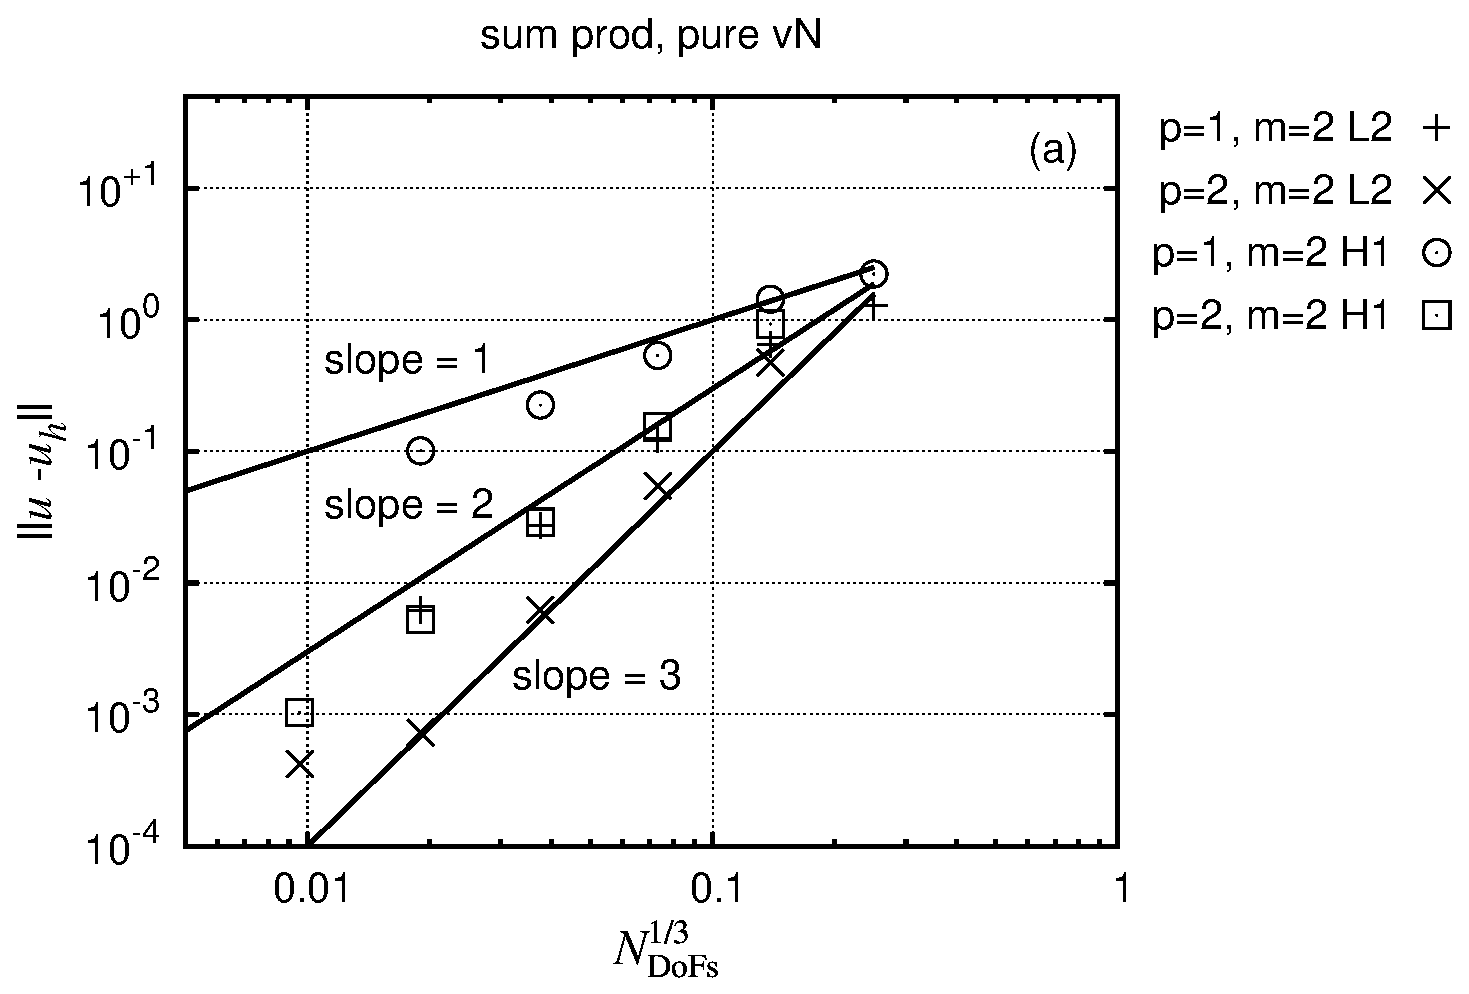
\includegraphics[angle=0, clip=true,
 % % % pdf % % %         trim=3cm 2.15cm 8.6cm 3.8cm,
    trim=0.1cm 1.9cm 5.5cm 1.3cm,
          width=0.435\textwidth]{DRS_FEM_BEM_wSciPAL_fig2a.eps}
           \label{DRS_FEM_BEM_wSciPAL-fig:conv-sum-prod-pvN}
          }
  % 
     \subfloat{
   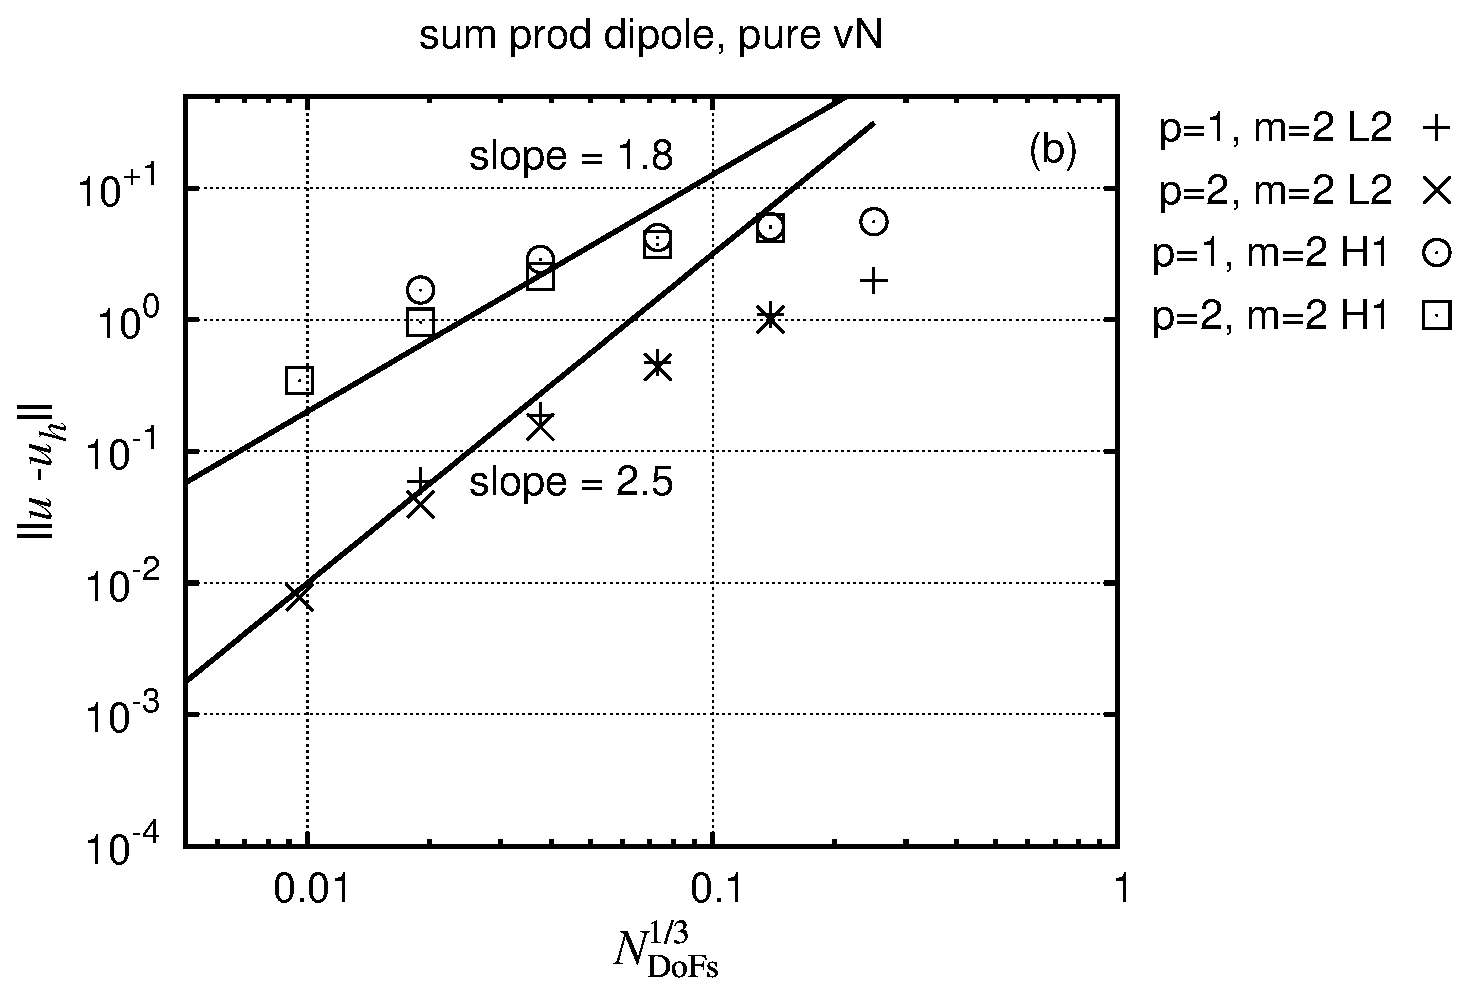
\includegraphics[angle=0, clip=true,
 % % % pdf % % %    trim=4.5cm 2.15cm 3.4cm 3.8cm,
   trim=2.8cm 1.9cm 0cm 1.3cm,
   width=0.5\textwidth]{DRS_FEM_BEM_wSciPAL_fig2b.eps}
    \label{DRS_FEM_BEM_wSciPAL-fig:conv-sum-prod-dipole-pvN}
   }
   \vspace{-.4cm}
   %
   %
 %%% \caption{Convergence of the pure Neumann problem, Eq.(\ref{DRS_FEM_BEM_wSciPAL-eq:pvN-testcase}).
 %%% %
 %%% (a) Harmonic test case, Eq.(\ref{DRS_FEM_BEM_wSciPAL-eq:sum-prod}).
 %%% %
 %%% (b) Dipole test case,  Eq.(\ref{DRS_FEM_BEM_wSciPAL-eq:sum-prod-dipole}). 
 %%% %
 %%% Both figures share y-axis labels and legend.
 %%%  %
 %%% }
  \label{DRS_FEM_BEM_wSciPAL-fig:convergence-pvN}
 %\end{figure}
 %\begin{figure}[htbp]
  %
    \subfloat{
     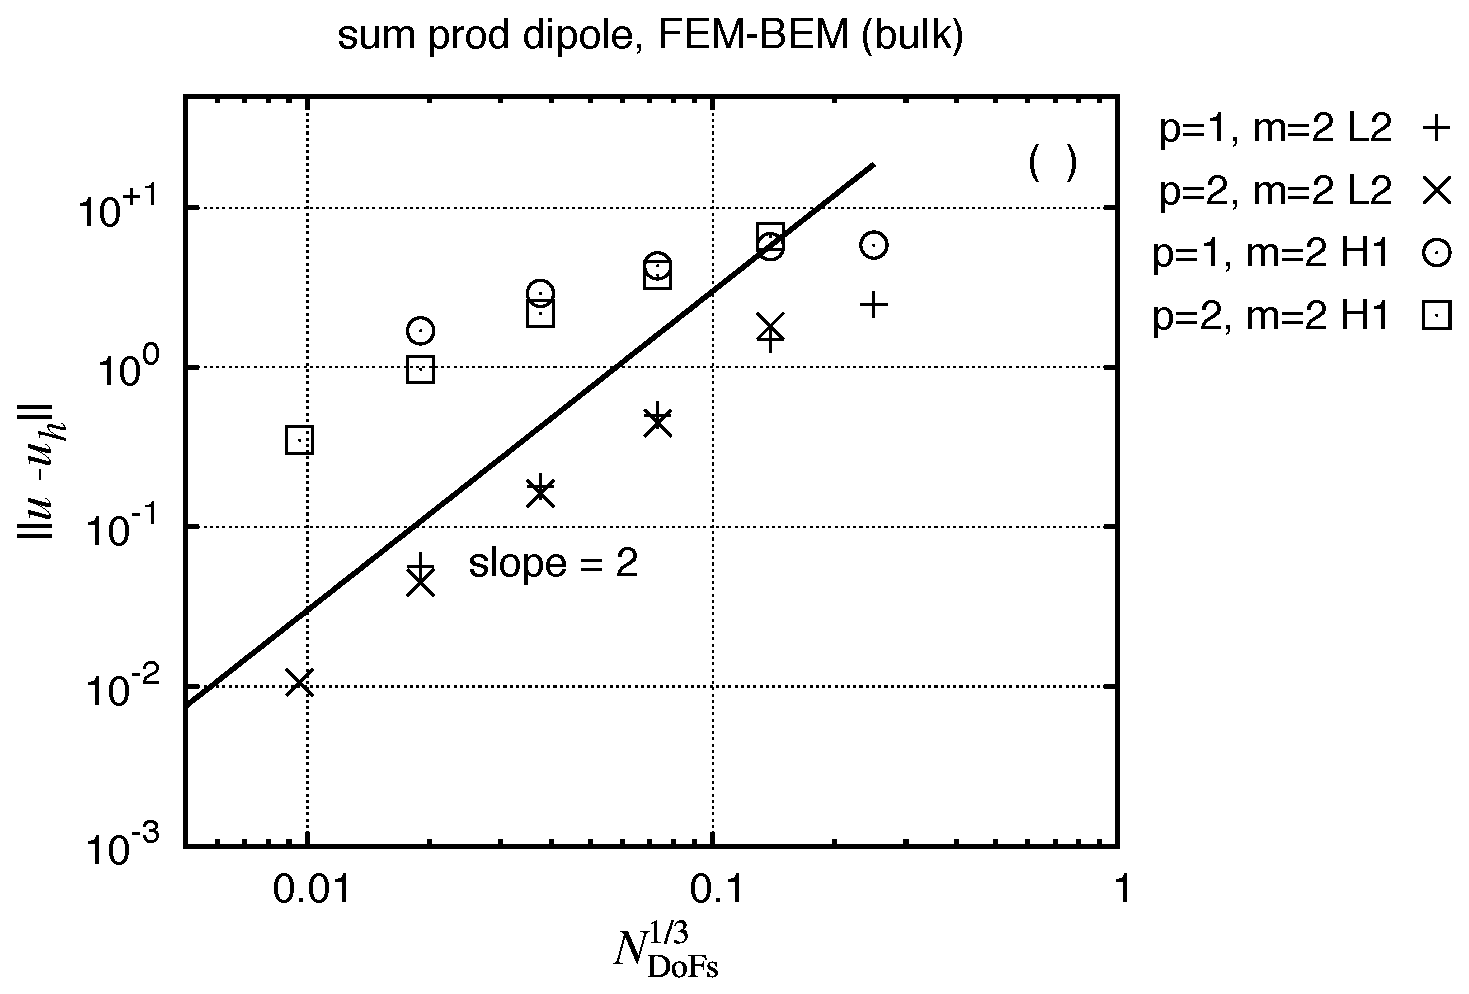
\includegraphics[angle=0, clip=true,
 % % % pdf % % %       trim=3cm 2.15cm 8.6cm 3.8cm,
    trim=0.1cm 0cm 5.5cm 1.3cm,
     width=0.435\textwidth]{DRS_FEM_BEM_wSciPAL_fig2c.eps}
      \label{DRS_FEM_BEM_wSciPAL-fig:pg-2}
     }
     %
        \subfloat{
         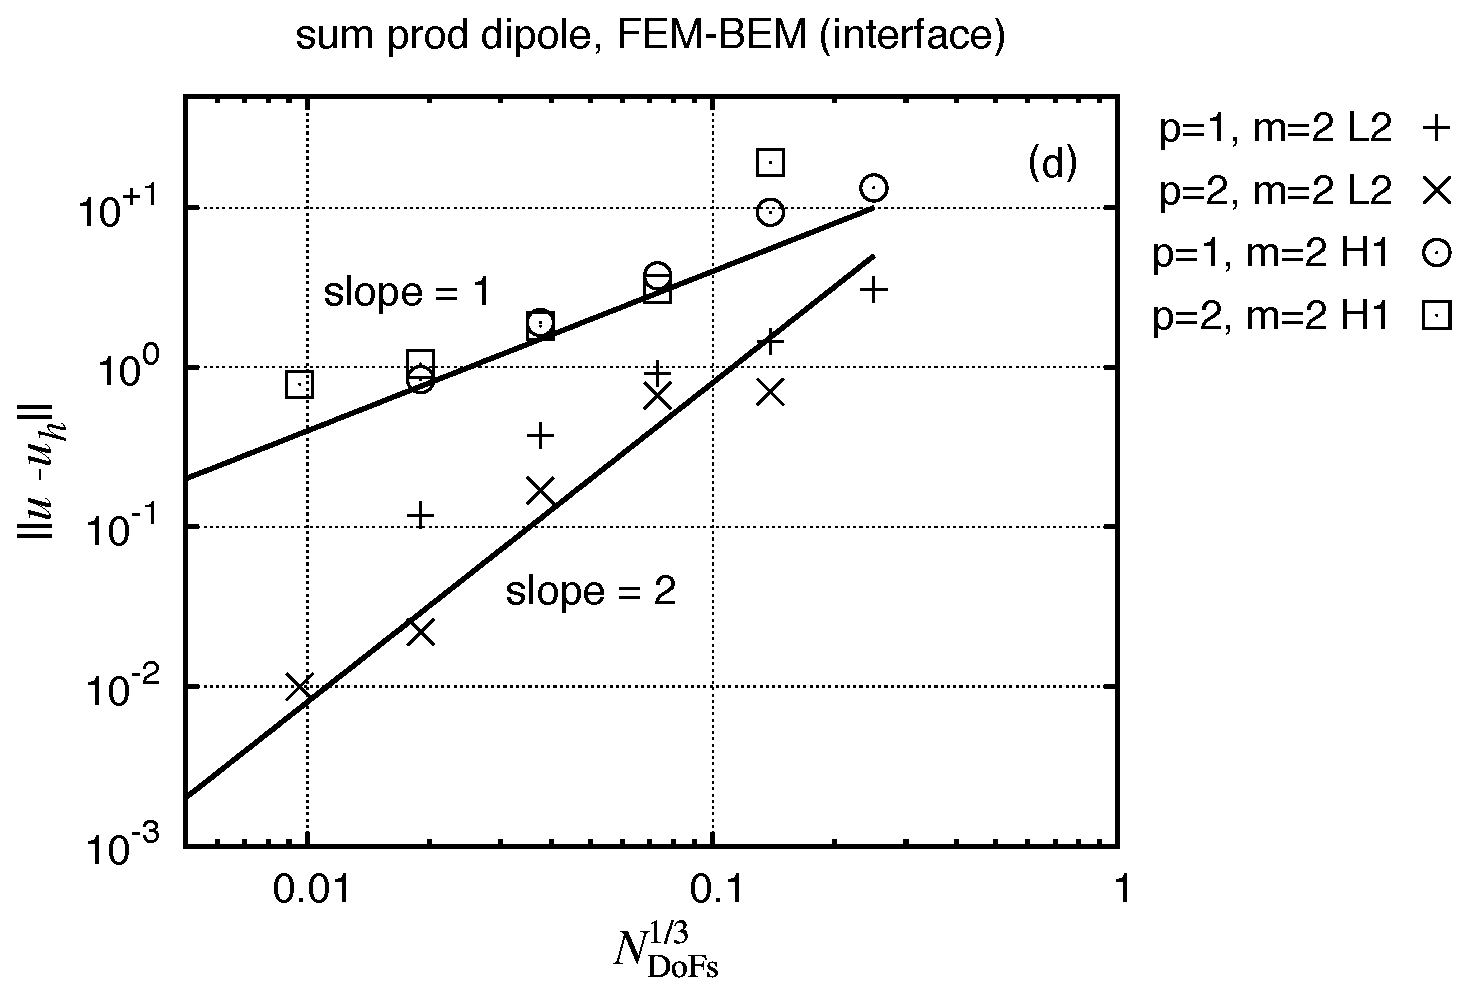
\includegraphics[angle=0, clip=true,
  % % % pdf % % %         trim=4.5cm 2.15cm 3.4cm 3.8cm,
    trim=2.8cm 0cm 0cm 1.3cm,
         width=0.5\textwidth]{DRS_FEM_BEM_wSciPAL_fig2d.eps}
          \label{DRS_FEM_BEM_wSciPAL-fig:pg-3}
         }
  %
  \caption{
 % % % post review change
 % Convergence of the pure Neumann problem, Eq.(\ref{DRS_FEM_BEM_wSciPAL-eq:pvN-testcase}).
 % (a) Harmonic test case, Eq.(\ref{DRS_FEM_BEM_wSciPAL-eq:sum-prod}).
 % (b) Dipole test case,  Eq.(\ref{DRS_FEM_BEM_wSciPAL-eq:sum-prod-dipole}). 
   Convergence of the Neumann problem, Eq.(\ref{DRS_FEM_BEM_wSciPAL-eq:pvN-testcase}), with (a) Eq.(\ref{DRS_FEM_BEM_wSciPAL-eq:sum-prod}), 
 (b) Eq.(\ref{DRS_FEM_BEM_wSciPAL-eq:sum-prod-dipole}) as solution. 
  %%% %
  %%% Both figures share y-axis labels and legend.
  %%%  %
  %%% }
  % % % post review change
  % Convergence of dipole test case,  Eq.(\ref{DRS_FEM_BEM_wSciPAL-eq:sum-prod-dipole}), on the FEM-BEM problem, Eq.(\ref{DRS_FEM_BEM_wSciPAL-eq:fem-bem-testcase}).
  % (a) FEM and (b) BEM error.
 (c) FEM and (d) BEM error for dipole test case, Eq.(\ref{DRS_FEM_BEM_wSciPAL-eq:sum-prod-dipole}), on the FEM-BEM problem, Eq.(\ref{DRS_FEM_BEM_wSciPAL-eq:fem-bem-testcase}).
   %
  %  (c) FEM and (d) BEM contributions to error of harmonic test case,  Eq.(\ref{DRS_FEM_BEM_wSciPAL-eq:sum-prod}).
  %Both f
  Figures share axis labels and legends.
  }
  \label{DRS_FEM_BEM_wSciPAL-fig:convergence-plots}
  %
 \end{figure}
%
\section{Results}
\label{DRS_FEM_BEM_wSciPAL-sec:drs-fem-bem-results}
%
\mydiff{In our tests we model the boundary piece-wise quadratically, $m=2$, which although not $C^1$-smooth, approximates the curved surface of a sphere sufficiently well. Hence, we do not have to care about}
{In our tests we model the boundary piece-wise by polynomials of order $m=2$, 
% % % post review change
% also explicitly stated in Figs.\ref{DRS_FEM_BEM_wSciPAL-fig:convergence-pvN} and\ref{DRS_FEM_BEM_wSciPAL-fig:convergence-plots}. 
cf. legend of Fig.\ref{DRS_FEM_BEM_wSciPAL-fig:convergence-plots}. 
%
This numerical boundary is not $C^1$-smooth. 
% % % post review change
%Yet, a
According to our tests, it approximates the curved surface of a sphere sufficiently well such that we do not have to consider}
%
the solid angle subtended by the surface elements at a vertex of the mesh of $\Gamma$.  
%
% % % post review change
% This is dictated by deal.II lacking the feature to assign different mappings to \mydiff{}{different} subboundaries. 
%
% % % post review change
% Because of
Due to 
 the outer surface of the DRS cell we cannot use the
 $C^1$-mapping provided by deal.II
 as deal.II cannot assign different mappings to \mydiff{}{different} subboundaries. 
 % 
 Throughout we use either linear ($p=1$) or quadratic ($p=2$) FEM.
 
 %
We are 
% % % post review change
% particularly 
interested in the convergence 
% % % post review change should be clear that it is te behavior
% behavior 
of our method for the pure Neumann problem and for the FEM-BEM coupling.
%
\mydiff{To this end, we}{We} define two 
% % % post review change
% simplified 
test problems with \mydiff{reference solutions}{solutions} 
\begin{eqnarray}
\label{DRS_FEM_BEM_wSciPAL-eq:sum-prod}
\Phi_{SP} & := & 0.1 (2x + y + z) + 0.01 xyz \,,  \\
%
\label{DRS_FEM_BEM_wSciPAL-eq:sum-prod-dipole}
\Phi_{D} & := &  \frac{1}{4 \pi |  {\bf x} - {\bf x}_+ | } -   \frac{1}{4 \pi |  {\bf x} - {\bf x}_- | } \,,
\end{eqnarray}
%
with $ {\bf x}_{\pm} = (0,0, \pm 0.5)$ in a sphere of radius 1.
%
As $\Phi_{ref}$ is either $\Phi_{SP} $ or $\Phi_{DSP} := \Phi_{D}  + \Phi_{SP}  $.
%
Note that $\Phi_{SP}$ is harmonic.
%
The  FEM-BEM convergence is assessed on the simplified problem: 
$find ~ (\Phi, t^P) \in X^{\Phi} \times Y ~ s.t. ~\forall  (\nu, \psi) \in X^{\Phi} \times Y' ~:$
%
\begin{subequations}
\label{DRS_FEM_BEM_wSciPAL-eq:fem-bem-testcase}
\begin{eqnarray}
 (\nabla v, \varepsilon_S \nabla \Phi)  
+
( v ,  \varepsilon_S t^P)_{\Gamma} & = &  0 \,,  \\
%
b_K(\psi_h, \Phi_h) % \left(\psi, \left(\frac 1 2  I  - K \right) \Phi \right)_{\Gamma}
    + 
     b_V(\psi_h,  t^P_h)
%  \left(\psi, \left(\frac 1 2  I  - K \right) \Phi \right)_{\Gamma} 
%    + 
%      \frac{\varepsilon_S}{\varepsilon_P}  \left(\psi,   V t^P \right)_{\Gamma}  
    & = & 
\left(\psi, \phi^C \right)_{\Gamma} \,, %\\
\end{eqnarray}
\end{subequations}
%
with $\Phi|_{\Gamma_A \cup \Gamma_0 \cup \Gamma_C} = \Phi_{ref} $.
%
%
The test for pure Neumann BCs is: $find ~ \Phi \in H^1(\Omega_S) ~s.t.$
%
\begin{eqnarray}
\label{DRS_FEM_BEM_wSciPAL-eq:pvN-testcase}
 (\nabla v, \nabla \Phi)  
 & = & 
( v ,  \partial_{\bf n}\Phi_{ref}  ) \quad \forall \nu \in  H^1(\Omega_S)  \,.
\end{eqnarray}
%
%
To measure the error we use the standard $L^2(\Omega_S)$- and $H^1(\Omega_S)$-norm
for the FEM part. 
%\begin{eqnarray}
%\label{L2-norm-vol}
%\| u - u_h\|^2_{L^2(\Omega_S)} & = & \int\limits_{\Omega_S} |u - u_h|^2 d \Omega_S \,, \\
%\nonumber \\
%\label{H1-norm-vol}
%\| u - u_h\|^2_{H^1(\Omega_S)} & = & \| u - u_h\|^2_{L^2(\Omega_S)}  + \int\limits_{\Omega_S} |\nabla u - \nabla u_h|^2 d \Omega_S \,.
%\end{eqnarray}
%
For the BEM part we measure the $L^2$ error of the trace of $\Phi$ on $\Gamma$
%\begin{eqnarray}
%\label{l2-norm-u-surf}
$
\| \Phi_{ref} - \Phi_h\|^2_{L^2(\Gamma)}  %=  (\Phi_{ref} - \Phi_h, \Phi_{ref} - \Phi_h)_{\Gamma} 
$, and the 
%
$L^2$ error in the trace of $\partial_n\Phi \equiv -t^P$ on $\Gamma$.
% % % post review change
% which we sloppily denote 
Here, denoted as $H^1(\Gamma)$ semi-norm
%\int_{\Gamma} |\Phi_{ref} - \Phi_h|^2 d \Gamma \,, 
% \\
%\nonumber \\
%\label{l2-norm-dnu-surf}
$ | \Phi_{ref} - \Phi_h |^2_{H^1(\Gamma)}  :=  \| \Phi_{ref} + t^P_h \|^2_{L^2(\Gamma)} $.
 %\int_{\Gamma} | \partial_n\Phi_{ref} - t_{P,h}|^2 d \Gamma
%\end{eqnarray}
%
In case of Eq.(\ref{DRS_FEM_BEM_wSciPAL-eq:pvN-testcase}) and $\Phi_{ref} = \Phi_{SP}$ convergence is as expected. 
%
%
For FEM of order~$p$ we get $\| u - u_h\|^2_{L^2(\Omega_S)} = O(h^{p+1})$ and $\| u - u_h\|^2_{H^1(\Omega_S)} = O(h^{p})$ independent of \mydiff{}{the order of the boundary approximation}~$m$, cf. Fig.\ref{DRS_FEM_BEM_wSciPAL-fig:conv-sum-prod-pvN}.
%
Figure~\ref{DRS_FEM_BEM_wSciPAL-fig:conv-sum-prod-dipole-pvN} shows that for $\Phi_{ref} = \Phi_{DSP}$ we roughly lose half an order which we attribute to the right-hand side of the BEM part containing the $\delta$-distributions for the point charges.
%
Figure \ref{DRS_FEM_BEM_wSciPAL-fig:pg-2} shows the convergence of the FEM part of Eq.(\ref{DRS_FEM_BEM_wSciPAL-eq:fem-bem-testcase}). 
%
% % % post review change
%Surprisingly, f
For \mydiff{}{Lagrange finite elements of order }$p=2$ the $L^2(\Omega_S)$ and $H^1(\Omega_S)$ error have the same asymptotic behavior.
%
The error in the BEM part, Fig.\ref{DRS_FEM_BEM_wSciPAL-fig:pg-3}, is as expected for linear elements ($p=1$). Due to the collocation the decay of the error in $t^P$ does not improve. 
%
% % % post review change
%However, t
The error of $\Phi|_{\Gamma}$ partly profits from higher order elements.
%
Figure \ref{DRS_FEM_BEM_wSciPAL-fig:drs-down} shows that
% % % post review change
%our simulations are able to resolve
local inhomogeneities of the cation density in the vicinity of the protein surface
% % % post review change
are resolved and
%
% % % post review change
% It also shows that
the current-carrying species (cations and neutral particles) are distributed opposite to each other.
%
\begin{figure}[ht]
\centering
% Use the relevant command for your figure-insertion program
% to insert the figure file.
% For example, with the graphicx style use
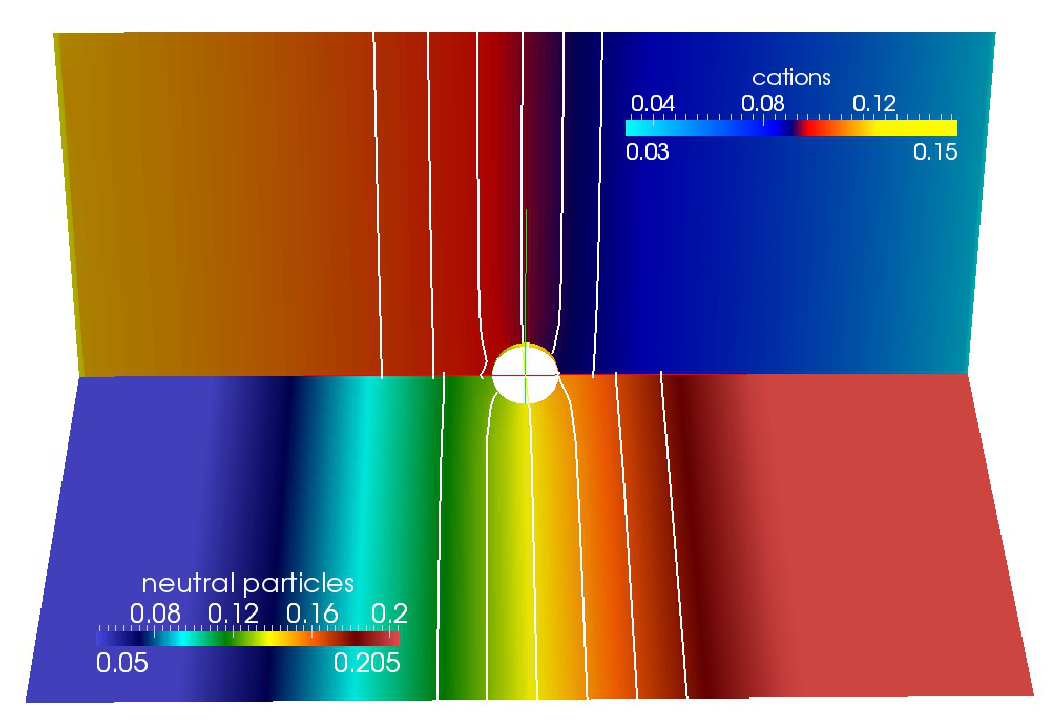
\includegraphics[clip=true,
% % % pdf % % % trim=2.3cm 17cm 1cm 1.9cm,
trim=0cm 1cm 0cm 0.7cm,
 width=.75\textwidth
 ]
 {DRS_FEM_BEM_wSciPAL_fig3_drs_ion_distribution_down.eps}
%
%If the width of the figure is less than 7.8 cm use the \texttt{sidecaption} command to flush the caption on
\caption{Distribution of cations and neutral particles in the DRS cell. }
\label{DRS_FEM_BEM_wSciPAL-fig:drs-down}    
\end{figure}

\section{Conclusion}
\label{DRS_FEM_BEM_wSciPAL-sec:drs-fem-bem-concl}
%

% % % post review change
To conclude, 
we have derived a mathematical model for the detailed simulation of the electro-diffusive processes in dielectric relaxation spectroscopy of proteins in solution including boundary effects inaccessible in previously derived stochastic models.
%
The key feature is the modeling of the protein-solvent interface as excluded volume with a smooth surface by taking into account its electrostatic properties by means of a boundary integral equation.
%
For the efficient solution of the resulting FEM-BEM model we have extended the geometric multigrid example of the deal.II library ({\sf step-16}) to vector-valued problems and higher order elements.
%
Unlike the strategy proposed in deal.II's  {\sf step-34} for boundary elements we have to use the traces of the finite elements as boundary elements.
%
Most of the equations in the DRS model are pure Neumann problems and subject to a conservation of particle numbers.
%
To assure their unique \mydiff{solubility}{solvability} we implemented an interleaved pseudo-time stepping / mesh refinement strategy which avoids the saddle-point problems arising from Lagrange multipliers. The convergence is as expected.
%
 The convergence of the FEM-BEM method depends on the particular test case but is consistent with the literature. 
%
 Applied to the full DRS problem our numerical results indicate the validity of the proposed explanation of the origin of the ``sub-$\beta$'' peak.


\section*{Appendix: A Posteriori Error Estimator for the External Current}

\subsection{DWR setup}

$B(.,.) : X \times Y \to \mathbb{R}$, bounded bilinear form, $F(.) : Y  \to \mathbb{R}$ bounded linear functional on test space, $J(.) : X  \to \mathbb{R}$ linear functional on trial space for measuring solution-dependent observables.

primal problem and associated dual problem
%
\begin{eqnarray}
\label{eq:prim-p}
find ~ u \in X ~: ~ B(u,v) & = & F(v) ~ \quad \forall v \in Y ~(prim.~prob.) \\
%
\nonumber \\
\label{eq:dual-p}
find ~ z \in X ~: ~ B(w,z) & = & J(w) ~  \quad \forall w \in X ~(dual~prob.) 
\end{eqnarray}

The primal solution $u$ is one particular $w$ in $X$ and $z$ is one particular $v$ in Y. 
%
Assuming a conformal discretization the same holds for the discrete solutions $u_h \in X_h \subset X$ and $z_h \in Y_h \subset Y$.
%
Therefore, Galerkin orthogonality $B(u-u_h, v_h) ~\forall v_h \in Y_h$ gives us for primal residual $R_p(u_h) \in Y' $
% 
\begin{eqnarray}
\label{eq:J-err}
J(u) - J(u_h) & = & B(u-u_h, z-z_h) \nonumber \\
&= & F(z-z_h) - B(u_h, z-z_h) \equiv \langle R_p(u_h), z-z_h  \rangle  
\end{eqnarray}
%
\begin{figure}[b]
%\sidecaption
% Use the relevant command for your figure-insertion program
% to insert the figure file.
% For example, with the graphicx style use
%\includegraphics[clip=true,
% trim=6.7cm 1.25cm 8.25cm 5cm,
% width=7cm]
 % {figures/drs-setup-and-effect.pdf}
%
%If the width of the figure is less than 7.8 cm use the \texttt{sidecaption} command to flush the caption on
\caption{DRS cell with subdomains $\Omega_P$ (protein interior) and $\Omega_S$ (solvent). 
%
The boundaries are $\Gamma$ (protein-solvent interface),  $\Gamma_A$ (anode), $\Gamma_C$ (cathode) and $\Gamma_0$ (impermeable hull of the DRS cell). 
%
The protein is modeled as a dipole consisting of two point charges immersed in a spherical, dielectric domain of relative permittivity $\varepsilon_P \approx 2$ while the aqueous surrounding has $\varepsilon_S \approx 80$. Depending on the intramolecular charge distribution, i.e.  conformation, of the protein a different number of ions is bound in the dielectric double layer at $\Gamma$. TO DO : use figreu from above}
\label{fig:drs-setup-and-effect-2}    
\end{figure}

\subsection{Physical problem}

We consider two coupled Laplace equations with homogeneous Neumann boundary conditions one of which will be solved by FEM and the other by BEM.
% 
For the geometric setup and the notation of the domain and its  boundaries cf. Fig.\ref{fig:drs-setup-and-effect-2}.
%
In the following ${\bf n}$ is always the outer normal of $\Omega_S$.
%
The continuous model is
%
\begin{eqnarray}
\label{eq:cats}
- \nabla^2 c_+ & = & 0 \quad \textrm{in} ~ \Omega_S, \\
%
{\bf n} \cdot \nabla c_+ & = & ~ - k_R~c_+  \quad \textrm{on} ~   \Gamma_C   \\
%
{\bf n} \cdot \nabla c_+ & = & ~ + k_O~c_0  \quad \textrm{on} ~   \Gamma_A   \\
%
{\bf n} \cdot \nabla c_+ & = & 0  \quad \textrm{on} ~   \Gamma \cup \Gamma_0 \\
\nonumber \\
- \nabla^2 c_0 & = & 0 \quad \textrm{in} ~ \Omega_S, \\
%
{\bf n} \cdot \nabla c_0 & = & ~ + k_R~c_+  \quad \textrm{on} ~   \Gamma_C   \\
%
{\bf n} \cdot \nabla c_0 & = & ~ - k_O~c_0  \quad \textrm{on} ~   \Gamma_A   \\
%
{\bf n} \cdot \nabla c_0 & = & 0  \quad \textrm{on} ~   \Gamma \cup \Gamma_0 
\end{eqnarray}
%
The cation density $c_+:\Omega_S \to \mathbb{R}$ and the density of the neutral particles $c_0:\Omega_S \to \mathbb{R}$ are assumed to be in the Sobolov space $H^1(\Omega_S)$.
%
$c_+$ will be computed from a finite element formulation (because in truth we still have to take into account the drift term $\nabla \cdot (c_+\nabla \Phi)$, $\Phi$ is the electrostatic potential generated from the charge distribution associated with the spatial distribution of the cations).
%
We still need some stuff for the boundary elements:

- $G_{\bf x}({\bf y}) := 1 / (4 \pi |  {\bf x} - {\bf y} | )  $
%
is the Green's function for the Laplace equation in three dimensions.
%

- To use the Johnson-N\'ed\'elec coupling~\cite{johnson1980coupling} we introduce the normal component of the densities w.r.t. to the outer normal of $\Omega_P$ as independent variable, i.e. w.r.t. to $\Omega_S$ it points inward
%
\begin{eqnarray}
t^P  & := & -\partial_{{\bf n}}\Phi \,.
\end{eqnarray}

- The single layer boundary integral operator $V : H^{-1/2}(\partial \Omega_S) \to H^{1/2}(\partial \Omega_S) $ and double layer boundary integral operator  $K : H^{1/2}(\partial \Omega_S) \to H^{1/2}(\partial \Omega_S) $ are defined as 
% 
\begin{eqnarray}
(V t^P)({\bf x}) & = & \oint\limits_{\partial \Omega_S}
%\left[
 G_{\bf x}({\bf x}')  % \frac{\varepsilon_S}{\varepsilon_P}  
   %\frac{\partial \Phi}{\partial{\bf n}'}
     t^P({\bf x}')
 %    \right] 
 d\Gamma ({\bf x}')  \,, \\
%
(K \Phi_P)({\bf x}) & = & % -
\oint\limits_{\partial \Omega_S}
%\left[
\frac{\partial G_{\bf x} }{\partial{\bf n}({\bf x}') }({\bf x}') 
 % \frac{\varepsilon_S}{\varepsilon_P}  
     \Phi({\bf x}')
  %   \right] 
 d\Gamma ({\bf x}')  \,.
\end{eqnarray}
%
The single layer boundary integral operator $V : H^{-1/2}(\partial \Omega_S) \to H^{1/2}(\partial \Omega_S) $ is bounded and $H^{-1/2}(\partial \Omega_S)$-elliptic and thus invertible.

- the restriction of the integral operators to the different subboundaries 

~~ - $K_0$ ($\Gamma_0 \cup \Gamma$) note that this is the union of two disjoint sets, cf. figure.

~~ - $K_A$, $V_A $ ($\Gamma_A$)

~ ~ - $K_C$ $V_C$ ($\Gamma_C$)

Our solution will be vector-valued
% $$u = (c_+, c_-\big|_{\Gamma_0 \cup \Gamma}, c_-\big|_{\Gamma_A}, c_-\big|_{\Gamma_C})$$ 
 $$u = (c_+, c^0_0, c^A_0, c^C_0)$$ 
 where the last three components are the traces of $c_-$ on the boundaries $\Gamma_0 \cup \Gamma$, $\Gamma_A$ and $\Gamma_C$, respectively. 
%
%The individual function spaces are
%% 
%\begin{eqnarray*}
%%
%c_+ & \in & H^1(\Omega_S) \\
%\\
% c_-\big|_{\Gamma_0 \cup \Gamma}  & \in & H^{1/2}(\Gamma_0 \cup \Gamma) \\
%% 
%\\
% c_-\big|_{\Gamma_A}  & \in & H^{1/2}(\Gamma_A) \\
% \\
%  c_-\big|_{\Gamma_C} & \in & H^{1/2}(\Gamma_C)
%%
%\end{eqnarray*}
%
Then, our combined function space should be 
%
$$  X :=  H^1(\Omega_S) \times H^{1/2}(\Gamma_C) \times H^{1/2}(\Gamma_0 \cup \Gamma)  \times H^{1/2}(\Gamma_A) . $$
%
The individual component spaces are Hilbert spaces, thus dual to itself and the dual of $X$ is $X$ again.
%
As shorthand notation for the individual subspace we introduce $X^S :=   H^1(\Omega_S)$,  $Y^C := H^{1/2}(\Gamma_C)$, $Y^A := H^{1/2}(\Gamma_A)$ and $Y^0 :=  H^{1/2}(\Gamma_0 \cup \Gamma)  $.
The Galerkin formulation of the coupled problem is
% 
\begin{eqnarray}
\label{eq:gal-form-prim-p}
(\nabla s, \nabla c_+)  + k_R  ( s,  c_+ )_{\Gamma_C} - k_O ( s,  c_0 )_{\Gamma_A} 
%
 & = & 0 \quad  \forall s \in H^1(\Omega_S) \,,   \\
 %
    - k_R \left( w,   V_C c_+\right)_{\Gamma_C} +   \left( w,  \left[ \frac 1 2 - K_C\right] c_0\right)  & = & 0 \quad  \forall w \in H^{1/2}(\Gamma_C)  \,, \\
 \nonumber \\
 \left( p,  \left[ \frac 1 2 - K_0 \right] c_0 \right)_{\Gamma_0 \cup \Gamma} & = & 0  \quad  \forall p \in H^{1/2}(\Gamma_0 \cup \Gamma)  \,, \\
 \nonumber \\
  \left( q,  \left[ \frac 1 2 - K_A + k_O V_A \right] c_0 \right)_{\Gamma_A}  & = & 0 \quad  \forall q \in H^{1/2}(\Gamma_A)  \,.
\end{eqnarray}
%
The bilinear form is formed by summing up all of the above equations.
%For the DWR setting $X = X$, $Y=X$ and 
The vector-valued test function is denoted as $v = (s, w, p, q) \in X^S \times Y^0 \times Y^A \times Y^C $.
%
Our target functional(s) is/are 
\begin{eqnarray}
J_+(u) & = &  k_R\int\limits_{\Gamma_C} c_+ ~d\Gamma_C \\
J_0(u) & = &  k_O\int\limits_{\Gamma_A} c_0 ~d\Gamma_A
\end{eqnarray}
%
$J_+$ measures the cation outflux at the cathode and $J_0$ the cation influx at the anode. Both are balanced by the corresponding fluxes of neutral particles. Hence, $J_+(u) + J_0(u) $ should be $0$.
%
%For the DWR setting $X = X$, $Y=X$ and the bilinear form is  
%%
%\begin{eqnarray}
%B(u, v) & = & 
%(\nabla s, \nabla c_+) - k_O ( s, c_0 )_{\Gamma_A}  + k_R ( s, c_+ )_{\Gamma_C} \nonumber \\
% &&  
%      -   k_R\left( w, V_C c_+\right)_{\Gamma_C}  +  \left( w,  \left[ \frac 1 2 - K_C\right] c_-\right)  \nonumber \\
%&& + 
% \left( p,  \left[ \frac 1 2 - K_0 \right] c_- \right)_{\Gamma_0 \cup \Gamma}\nonumber \\
% && +
%   \left( q,  \left[ \frac 1 2 - K_A + k_O V_A \right] c_- \right)_{\Gamma_A}
%\end{eqnarray}
%
%The test function is $v = (s, w, p, q)$.
%

The dual problems can formally identified by comparing Eqs.~(\ref{eq:dual-p}) and (\ref{eq:gal-form-prim-p}ff).

For the primal residual we have to integrate by parts again cell-wise in the FEM part ($T \subset \Omega_S$ is a cell and $\partial T $ its boundary, $[...]$ are jumps, the dual solution is $z = (z^+, z^{C},  z^{0},  z^{A} )$)
%
\begin{eqnarray}
J(u-u_h) =  B(u, z-z_h) & = & \sum_T \left\lbrace
( z^+ - z^+_h, - \nabla^2 c_+)_{T}  +  \frac 1 2 (z^+ - z^+_h, [\partial_{\bf n} c_+] )_{\partial T} \right\rbrace \nonumber \\
\nonumber \\
&&   - ( z^+ - z^+_h, k_O c_0 )_{\Gamma_A}  + ( z^+ - z^+_h,  k_R c_+ )_{\Gamma_C} \nonumber \\
 \nonumber \\
 &&  +
     \left( z^C - z^C_h,  \left[ \frac 1 2 - K_C\right] c_-\right)    - \left( z^C - z^C_h,  k_R V_C c_+\right)_{\Gamma_C}   \nonumber \\
\nonumber \\
&& + 
 \left( z^0 - z^0_h,  \left[ \frac 1 2 - K_0 \right] c_- \right)_{\Gamma_0 \cup \Gamma}\nonumber \\
 \nonumber \\
 && +
   \left( z^A - z^A_h,  \left[ \frac 1 2 - K_A + k_O V_A \right] c_- \right)_{\Gamma_A}
\end{eqnarray}



\subsection{Discretization}

We solve by successive local refinement. This introduces a sequence of finite-dimensional subspaces ${X_h} \subset X$, parametrized by the cell diameter $h$.
%
For both the primal and dual problem we use deal.II's class\verb|FE_Q<dim>| for globally continuous Lagrange elements. 
%
For the primal problem we use linear elements and for the dual one we use quadratic elements. Otherwise the dual weights $z -I_h z$ would vanish. The ``true" solution $z$ is approximated by higher finite elements and $I_h z$ is the interpolation into the finite element space of the primal problem which is of lower dimension.
%
Formally, due to its larger number of degrees of freedom (DoFs), the dual FE space can be considered of having a finer mesh width than the primal FE space. Therefore, we denote the former as $X_h$ and the latter as $X_H$ with $H= 2h$.
%
The discrete problems are then 
%
\begin{eqnarray}
\label{eq:prim-p-fe}
find ~ u_H \in X_H ~: ~ B(u_H,v_H) & = & F(v_H) ~ \quad \forall v_H \in X_H \\
%
\nonumber \\
\label{eq:dual-p-fe}
find ~ z_h \in X_h ~: ~ B(w_h,z_h) & = & J(w_h) ~  \quad \forall w_h \in X_h  
\end{eqnarray}
%
In contrast to FE-only computations we have to cope with the problem of the double integrals in the discretizations of the integral operators. The double integration is avoided by using the support points of the finite element functions as collocation points.
%
With $t^P_h = \sum_i t^P_i \phi_i$, e.g. the entries $V_{ij}$ of the matrix representing the single layer operator are formally given by
$$
V_{ij} = (\phi_i , V \phi_j ).
$$ 
Let ${\bf x}_i$ be the support point of DoF~$i$, then collocation at ${\bf x}_i$ can be interpreted as 
$$
V_{ij} = (\delta ({\bf x} - {\bf x}_i) , V \phi_j ).
$$ 
Thus, $V_{ij}$ and $K_{ij}$ are computed from 
\begin{eqnarray}
V_{ij} & = & \oint\limits_{\partial \Omega_S}
%\left[
 G_{{\bf x}_i}({\bf x}') 
     \phi_j({\bf x}')
 %    \right] 
 d\Gamma ({\bf x}')  \,, \\
%
K_{ij} & = & % -
\oint\limits_{\partial \Omega_S}
\frac{\partial G_{{\bf x}_i} }{\partial{\bf n}({\bf x}') }({\bf x}') 
     \phi_j({\bf x}')
 d\Gamma ({\bf x}')  \,.
\end{eqnarray}

The matrices for the dual problem are obtained by using the transpose.

problems:
\begin{itemize}
\item BEM stuff to be computed with collocation; as collocation points the support points of the FEM DoFs are used
\item does collocation spoil e.g. Galerkin orthogonality or render other assumptions invalid/unusable?
\item what exactly is the dual problem?
\item well-posedness of the primal problem itself. How should the equation for $c_0$ ever detect changes in the global average? How does this pop up again in the boundary integral formulation?
\end{itemize}
\newpage









%
%\bibliographystyle{vmams}  
%   % use BibTeX file example.bib (BibTeX -> author.bbl)
%\bibliography{../../../Doktorarbeit/diss}


\ifx\undefined\bysame
\newcommand{\bysame}{\leavevmode\hbox to3em{\hrulefill}\,}
\fi
\begin{thebibliography}{99}
\parskip1.0ex


\bibitem{kremer2003broadband}
  {\sc F. Kremer and A. Sch{\"o}nhals},
{\em Broadband Dielectric Spectroscopy}, Springer, % Berlin Heidelberg, 
2003.




\bibitem{Knocks2001}
{\sc A.~Knocks and H.~Weing{\"a}rtner}, 
{\em The dielectric spectrum of ubiquitin in aqueous solution},
 The Journal of Physical Chemistry B, {\bf 105}:17 (2001), 3635--3638.

%2
\bibitem{BanAngewChemIE2011}
{\sc D.~Ban et al.}, {\em Kinetics of
  conformational sampling in ubiquitin}, Angewandte Chemie International
  Edition {\bf 50}:48 (2011), 11437--11440.
  
  %6
  \bibitem{kleanthous2000protein}
  {\sc C.~Kleanthous},  {\em Protein-protein Recognition}, % Frontiers Series, 
  Oxford University Press, 2000.
  
 

%4
\bibitem{JanssenKanschat2011SIAM}
{\sc B.~Janssen and G.~Kanschat}, {\em Adaptive multilevel methods with local
  smoothing for $H^1$- and $H^{\mathrm{curl}}$-conforming high order finite
  element methods}, SIAM Journal on Scientific Computing {\bf 33}:4 (2011),
  2095--2114.
  
  %3
  \bibitem{dealii2007}
  {\sc W.~Bangerth, R.~Hartmann, and G.~Kanschat}, {\em {deal.II} -- a general
    purpose object oriented finite element library}, ACM Trans. Math. Softw. {\bf
    33}:4 (2007), 24/1--24/27.

%9
\bibitem{schmickler2010interfacial}
{\sc W.~Schmickler and E.~Santos}, {\em Interfacial electrochemistry},
  Springer, 2010.
  
  %7
  \bibitem{kramer2012cuda}
  {\sc S.~C. Kramer}, {\em Cuda-based scientific computing - tools and selected
    applications}, Ph.D. thesis, 
    %Institut f{\"u}r Angewandte und Numerische Mathematik, 
    Georg-August Universit{\"a}t G{\"o}ttingen, 2012.
  
   
  %1
  \bibitem{Bajaj20091684}
  {\sc C.~L. Bajaj, G.~Xu, and Q.~Zhang}, {\em A fast variational method for the
    construction of resolution adaptive {$C^2$}-smooth molecular surfaces},
    Computer Methods in Applied Mechanics and Engineering {\bf
    198}:21 (2009), 1684 -- 1690.
    %, Advances in Simulation-Based Engineering Sciences Honoring J. Tinsley Oden.
  

%8
\bibitem{Rjasanow2007book}
{\sc S.~Rjasanow and O.~Steinbach}, {\em The fast solution of boundary integral
  equations% (Mathematical and analytical techniques with applications to engineering)
   }, Springer, %-Verlag New York, Inc., Secaucus, NJ, USA, 
   2007.


%5
\bibitem{johnson1980coupling}
{\sc C.~Johnson and J.~N{\'e}d{\'e}lec}, {\em On the coupling of boundary
  integral and finite element methods}, Math. Comp {\bf 35}:152 (1980),
  1063--1079.

%10
\bibitem{steinbach2007numerical}
{\sc O.~Steinbach},  {\em Numerical Approximation Methods for Elliptic Boundary Value
  Problems}, Texts in Applied Mathematics, Springer, 2007.


\end{thebibliography}

\end{document}
